\documentclass[a4paper]{jpconf}
\usepackage{graphicx}
\usepackage{comment}
\usepackage{cite}
\usepackage{gensymb}
\usepackage{epstopdf}
\usepackage{amsmath}
\usepackage{amssymb} 	%for symbols
\usepackage[colorlinks,bookmarksopen,bookmarksnumbered,allcolors=blue]{hyperref}

\graphicspath{{./figures/}}

\begin{document}
\title{Validation of an Actuator Line Model Coupled to a Dynamic Stall Model for
Pitching Motions Characteristic to Vertical Axis Turbines}


\author{Victor Mendoza$^{1}$, Peter Bachant$^{2}$, Martin Wosnik$^{2}$ and Anders Goude$^{1}$ }
\address{$^{1}$ Department of Engineering Sciences, Division of Electricity, Uppsala University, \\Uppsala 751 21, Sweden}
\address{$^{2}$ Center for Ocean Renewable Energy, University of New Hampshire, 24 Colovos Rd.,\\ Durham, NH 03824, USA}
\ead{victor.mendoza@angstrom.uu.se}

\begin{abstract}
    Vertical axis turbines (VATs) can be used to extract renewable energy from
    wind or water flows. A simpler design, low cost of maintenance, and the
    ability to accept flow from all directions perpendicular to the rotor axis
    are some of the most important advantages over conventional horizontal axis
    turbines (HATs). However, VATs encounter complex and unsteady fluid
    dynamics, which present significant modeling challenges. One of the most
    relevant phenomena is dynamic stall, which is caused by the unsteady
    variation of angle of attack throughout the blade rotation, and is the focus
    of the present study. Dynamic stall is usually used as a passive control for
    VAT operating conditions, hence the importance of predicting its effects. In
    this study, a coupled model is implemented with the open-source CFD
    toolbox OpenFOAM for solving the Navier--Stokes equations, where an actuator
    line model and dynamic stall model are used to compute the blade loading and
    body force. Force coefficients obtained from the model are validated with
    experimental data of pitching airfoil in similar operating conditions as an
    H-rotor type VAT. Numerical results show reasonable agreement with
    experimental data for pitching motion.
\end{abstract}

\section{Introduction}

Operating conditions of Vertical Axis Wind Turbines VAWTs are characterized as
complex unsteady flows which give a considerable challenge, both to describe
using measurements and to represent through simulation
tools~\cite{huyer1996unsteady}. Moreover, VAWT blades are inherently exposed to
cyclic variation in the angle of attack, which gives cyclic blade forces and can
give material fatigue damage. Accurate modeling of the varying forces is
therefore very important for the design of the VAWT.

The amplitude of the angle of attack oscillation in a fixed pitch VAWT is
increasing with decreased tip speed ration (TSR), and at low TSR (common during
stall regulation), the blades will experience dynamic stall, where the force
coefficients for the blade not only depend on the angle of attack, but also on
the rate of change of the angle of attack. The aim of this study is to
investigate the performance of a Leishman-Beddoes type dynamic stall model when
implemented within an actuator line model, for pitching motion typical to a
VAWT.


\section{Methodology}

For solving the governing equations of the phenomena involved, a coupled model
has been implemented: the actuator line model (ALM) samples the flow velocity
from the Navier--Stokes solver, and thereby computes each blade element's angle
of attack and relative velocity. The dynamic stall model is used to calculate
blade force coefficients, which the actuator line model uses to impart the body
force back into the flow solver.

In this work, it was chosen to validate the model against wind tunnel data for a
pitching blade. This will put the focus on the force modeling part in the
simulation model.

\subsection{Actuator Line Model}

The ALM is a three-dimensional and unsteady aerodynamic model developed by
S{\o}rensen and Shen\cite{sorensen1999computation}, used to study the flow
around wind turbines. It is a combination of a solver of the Navier--Stokes equations
with a so-called actuator line technique, in which blades of the turbine are
represented by a distribution of body forces along lines. These forces
are determined using a dynamic stall model commonly based on empirical data.
This work uses the library turbinesFoam developed by Bachant et
al.~\cite{bachant2015simulating,Bachant2016-VAT-ALM,turbinesFoam-v0.0.7}.

The model employed here is based on the incompressible Navier--Stokes equation
\begin{align}
 & \nonumber \\ & \dfrac{\partial \vec{V}}{\partial t} + \vec{V} \cdot \nabla \vec{V} = - \dfrac{1}{ \rho} \nabla p + \nu \nabla ^2 \vec{V} + \vec{f}	  \label{eqmom}
\end{align} %\begin{align}
with $\vec{f}$ representing the body forces, which are the loads on the rotating blades for this case.

Static lift and drag coefficients of the 2D profile used for this study are
taken from the technical technical report made by Sheldahl and Klimas
\cite{sheldahl1981aerodynamic}, which is a popular database containing values
for a wide range of Reynolds numbers. These coefficients are tabulated and
combined with the blade element approach for determining body forces acting on
blades. Relative flow velocity $\vec{V}_{\mathrm{rel}}$ and angle of attack
$\alpha$ are calculated for each blade using the geometric relation between the
velocity of the blade $- \omega r$, with $\omega$ representing the angular
(rotational) velocity of the rotor and $r$ the radius of the blade element, and
the velocity of the local incoming wind flow $\vec{V}_{\mathrm{in}}$. Figure
\ref{figvectors} depicts a cross-sectional airfoil element at radius $r$ in the
plane perpendicular to the turbine axis.

\begin{figure}[h]
%\begin{minipage}{36pc}
\begin{center}
\includegraphics[width=0.35\columnwidth]{vector.eps}
\end{center}
%\resizebox{\columnwidth}{!}{\input{plot}}
%\end{minipage}%
\caption{\label{figvectors} Illustration of velocity vectors and forces acting at the cross-section airfoil element}
\end{figure}

Once the angle of attack, relative velocity are obtained, the blade element lift and drag forces per spanwise length unit are calculated as
\begin{align}
& f_L = \frac{1}{2} \ \rho \ c \ C_L \left| V_{\mathrm{rel}} \right|^2  \label{lift}
\end{align} %\begin{align}
\begin{align}
& f_D = \frac{1}{2} \ \rho \ c \ C_D \left| V_{\mathrm{rel}} \right|^2  \label{drag}
\end{align} %\begin{align}
where $C_L$ and $C_D$ are the lift and drag coefficients, respectively. Both are
function of the Reynolds number and the angle of attack. It should be emphasized
that the direction of the lift and drag are respectively perpendicular and
parallel to the relative velocity $\vec{V}_{\mathrm{rel}}$. $c$ represents the
chord length.

Same procedure is used to calculate forces from the turbine shaft and blade
support struts. After all these forces on the actuator lines are calculated,
then are added as a body force source, per unit of density (incompressible
assumption), in the momentum Navier--Stokes equations (equation \ref{eqmom}).


\subsection{Dynamic Stall Modeling}

The dynamic stall model (DSM) is represented by the Leishman-Beddoes
model~\cite{leishman1986generalised} with the modifications of Sheng et
al.~\cite{sheng2008modified} and Dyachuk~\cite{dyachuk}. It is capable to
calculate the unsteady lift, pitching moment and drag, giving a physical
description of the aerodynamics. It have been validated with experimental data
in~\cite{leishman1989semi}. The model is separated into three subsystems: an
attached flow model for unsteady linear airloads, a separated flow model for
non-linear airloads and a dynamic stall model for the airloads induced by the
leading edge vortex.

The unsteady attached flow solution considers the circulatory and impulsive loads, which, at the same time depend on the unsteady bound vortex. The circulatory normal force coefficient could be expressed as
\begin{align}
& C_{N_n}^C = C_{N_\alpha} \alpha_{E_n}	\label{CNcirc}
\end{align}
where $C_{N \alpha}$ indicates the slope of the static normal force coefficient for a specific Reynolds number, and $\alpha_{E_n}$ is an expression for an equivalent angle of attack
\begin{align}
& \alpha_{E_n} = \alpha_n - X_n -Y_n - Z_n	\label{alphaeq}
\end{align}
where $\alpha$ is the geometrical angle of attackm $X$, $Y$ and $Z$ are the deficiency functions, which are empirically derived, based on the flow velocity and the pithing rate, the details are found in \cite{dyachuk2013dynamic}. Indices $n$ and $n-1$ in equations \ref{CNcirc} and \ref{alphaeq} represent the current and previous time-step. A delayed angle of attack is considered due to the lag in pressure response, and it is calculated as
\begin{align}
& {\alpha _n}' = {\alpha _n} - D_{\alpha _n}    	\label{alphadel}
\end{align}
with $D_\alpha$ as the deficiency function
\begin{align}
& D_{\alpha_n} = D_{\alpha_{n-1}} \exp \left( - \frac{\Delta s}{T_\alpha} \right) + (\alpha_n - \alpha_{n-1})\exp \left( - \frac{\Delta s}{2T_\alpha} \right) \label{defalpha}
\end{align}
with the empirically derived time constant $T_\alpha$, which has a value of $T_\alpha$ = 6.3 for the NACA0021 airfoil, and $\Delta s$ corresponds to a non-dimensional time-step
\begin{align}
& \Delta s = \frac{2 | \vec{V}_{rel} | \Delta t}{c}		.	\label{deltas}
\end{align}

Because of the reversal flow in the boundary layer, a leading edge vortex is created at the surface of the airfoil. The critical angle of attack $\alpha_{cr_n}$ defines the condition at which dynamic stall begins
\begin{align}
\alpha_{cr_n} =
\begin{cases}
    \alpha_{ds0}       & \quad |r_n| \geqslant r_0 \\
    \alpha_{ss} + (\alpha_{ds0} - \alpha_{ss}) \frac{| r_n |}{r_0}       & \quad |r_n| < r_0 \\
\end{cases}		\label{criticalpha}
\end{align}
with the reduced pitching rate $r_n$ defined as
\begin{align}
r_n = \frac{\dot{\alpha}_n c}{ 2 | \vec{V}_{rel} | }
\end{align}
here, $\dot{\alpha}$ is the pitch rate, $r_0$ is the reduced pitching rate, which limits the quasi-steady stall with the dynamic stall. Its value is $r_0$ = 0.01 for the NACA0021 airfoil. The static stall onset angle $\alpha_{ss}$ and the critical stall onset angle $\alpha_{ds0}$ are 14.33 and 17.91, respectively. The following is the the dynamic stall condition used
\begin{align}
| \alpha ' | > \alpha_{cr} \rightarrow \mathrm{stall} \label{stall}
\end{align}
for the separated flow, the effects are divided in two groups: trailing edge separation and leading vortex convection. The first one is related to the time delay in the movement of the boundary separation point, and is calculated using Kirchhoff's approximation
\begin{align}
f'_n =
\begin{cases}
    1- 0.4 \exp \left( \frac{|\alpha'_n| - \alpha_1 }{S_1}   \right)    & \quad |\alpha'_n| <  \alpha_1 \\
    0.02- 0.58 \exp \left( \frac{\alpha_1 - |\alpha'_n| }{S_2} \right)  & \quad |\alpha'_n| \geqslant  \alpha_1 \\
\end{cases}		\label{criticalpha2}
\end{align}
where $f'$ is the delayed separation point and $\alpha_1$, $S_1$ and $S_2$ are constant based on the airfoil profile and the local Reynolds number, these can be found in \cite{dyachuk2013dynamic}. The boundary layer around the blade is in function on the time, and this effect is superimposed on the pressure response delay. The additional delay is represented by $f''$, which is the dynamic separation point
\begin{align}
f''_n = f'_n - D _{f_n}	   \label{dyndelay}
\end{align}
and $D_{f_n}$ is the deficiency function defined as
\begin{align}
& D_{f_n} = D_{f_{n-1}} \exp \left( - \frac{\Delta s}{T_f} \right) + (f_n - f_{n-1})\exp \left( - \frac{\Delta s}{2T_f} \right) \label{deff}
\end{align}
Here, $T_f$ is empirically derived time constant and its value is $T_f$ = 3. Then, the normal force coefficient for unsteady conditions before the dynamic stall onset is calculated as
\begin{align}
& C_{N_n}^f = C_{N_\alpha} \alpha_{E_n} \left( \frac{1 + \sqrt{f''}}{2} \right)^2	\label{CNf}
\end{align}
after the stall condition is met, the leading edge vortex convects over the surface of the airfoil towards the trailing edge. A significant increase in the normal forces occurs during this process
\begin{align}
C_N^v = B_1 (f'' - f) V_x \label{CNv}
\end{align}
where $C_N^v$ represents the normal force coefficient during the vortex convection, which is in function of the pitch rate. $V_x$ and $B_1$ are parameters based on the local Reynolds number and the airfoil profile, they are found in \cite{dyachuk2013dynamic}. Once the vortex passes the trailing edge, the normal force decreases quickly. Total normal force obtained is expressed as
\begin{align}
C_N = C_{N_n}^f + C_N^v \label{CNtotal}
\end{align}
Figure \ref{figpitching} shows an example of the normal coefficient forces on a blade during pitching motion, using the above model described.

\begin{figure}[h]
%\begin{minipage}{36pc}
\begin{center}
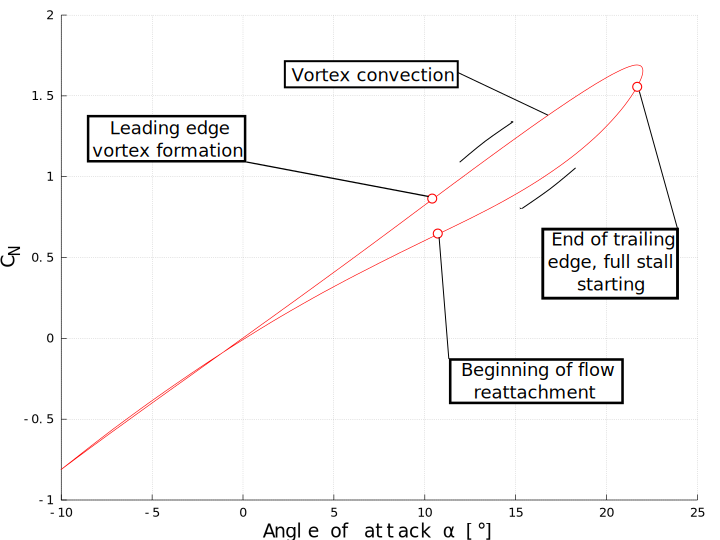
\includegraphics[width=0.5\columnwidth]{CNpitching2.eps}
\end{center}
%\resizebox{\columnwidth}{!}{\input{plot}}
%\end{minipage}%
\caption{\label{figpitching} Illustration of dynamic stall: NACA0021 profile with $\alpha=6 + 16 \sin (\omega	t), \ \omega=12,47$ [rad/s], $V_\infty=34,3$ [m/s] and $c$ = 0,55[m]}
\end{figure}

Tangential force coefficient is calculated trough Kichhoff's flow relation using the dynamic separation point.
\begin{align}
C_T = \eta C_{N_\alpha} \alpha_E ^2 ( \sqrt{f''}-E_0)     \label{CT}
\end{align}
with the empirical constants $\eta = 0.975$ and $E_0 = 0.15$ corresponding to NACA0021 airfoil profile.





\section{Simulation Parameters: Validation case}
A NACA0021 airfoil was tested at the Reynolds number of 1.000.000 (which is a
reasonable value for operating VAWT) during pitching motion similar to the motion
of the VAWT blade. Different pitching amplitudes were investigated: 13.8, 17.4 and 22.6$\degree$, analog to a TSR of $\lambda=$ 4.19, 3.34 and 2.6 respectively (see equation \ref{tsrval}), to cover a wide range of operational conditions of a VAWT.  In a VAWT with
fixed blades, the angle of attack is in function of the TSR of the turbine. A
periodic function is used to represent the variations of the angles of attack
which a VAWT blade experiences analog to the pitching motion,
\begin{eqnarray}
    \alpha = \arctan \left( \frac{\sin \theta}{\lambda + \cos \theta} \right) \label{alphaval}
\end{eqnarray}
where $\theta$ is the azimuthal blade angle and $ \lambda $ represents the TSR,
\begin{eqnarray}
    \lambda =  \frac{\Omega R}{ |\vec{V}_\infty | } \label{tsrval}
\end{eqnarray}
In the equation \ref{alphaval}, $\alpha$ represents the geometric angle of attack, and it is different to the effective angle of attack $\alpha_E$, which is calculated by the model in order to get the force coefficients. A NACA0021 profile with 0.55 [m] of chord length is driven to the dynamic stall region trough the pitching motion accordint to equation \ref{alphaval}. The pitching blade experiments were carried out at Glasgow
University\cite{angell1988collected}.



\section{Results and discussion}
In this section, obtained results for $C_N$ and $C_T$ from simulations are compared with the experimental data. Varying parameters have been tested, mainly in the deep stall condition for an amplitude of 22.6 $\degree $ (equivalent to $\lambda$ = 2.6). All the studied cases were simulated using a LES Smagorinsky turbulence model. Figure \ref{revolutions} shows that the model needs two revolutions to reach the convergence, a third revolution will not produce any change.

\begin{figure}[h]
\begin{minipage}{18pc}
\resizebox{\columnwidth}{!}{% GNUPLOT: LaTeX picture with Postscript
\begingroup
  \makeatletter
  \providecommand\color[2][]{%
    \GenericError{(gnuplot) \space\space\space\@spaces}{%
      Package color not loaded in conjunction with
      terminal option `colourtext'%
    }{See the gnuplot documentation for explanation.%
    }{Either use 'blacktext' in gnuplot or load the package
      color.sty in LaTeX.}%
    \renewcommand\color[2][]{}%
  }%
  \providecommand\includegraphics[2][]{%
    \GenericError{(gnuplot) \space\space\space\@spaces}{%
      Package graphicx or graphics not loaded%
    }{See the gnuplot documentation for explanation.%
    }{The gnuplot epslatex terminal needs graphicx.sty or graphics.sty.}%
    \renewcommand\includegraphics[2][]{}%
  }%
  \providecommand\rotatebox[2]{#2}%
  \@ifundefined{ifGPcolor}{%
    \newif\ifGPcolor
    \GPcolorfalse
  }{}%
  \@ifundefined{ifGPblacktext}{%
    \newif\ifGPblacktext
    \GPblacktexttrue
  }{}%
  % define a \g@addto@macro without @ in the name:
  \let\gplgaddtomacro\g@addto@macro
  % define empty templates for all commands taking text:
  \gdef\gplbacktext{}%
  \gdef\gplfronttext{}%
  \makeatother
  \ifGPblacktext
    % no textcolor at all
    \def\colorrgb#1{}%
    \def\colorgray#1{}%
  \else
    % gray or color?
    \ifGPcolor
      \def\colorrgb#1{\color[rgb]{#1}}%
      \def\colorgray#1{\color[gray]{#1}}%
      \expandafter\def\csname LTw\endcsname{\color{white}}%
      \expandafter\def\csname LTb\endcsname{\color{black}}%
      \expandafter\def\csname LTa\endcsname{\color{black}}%
      \expandafter\def\csname LT0\endcsname{\color[rgb]{1,0,0}}%
      \expandafter\def\csname LT1\endcsname{\color[rgb]{0,1,0}}%
      \expandafter\def\csname LT2\endcsname{\color[rgb]{0,0,1}}%
      \expandafter\def\csname LT3\endcsname{\color[rgb]{1,0,1}}%
      \expandafter\def\csname LT4\endcsname{\color[rgb]{0,1,1}}%
      \expandafter\def\csname LT5\endcsname{\color[rgb]{1,1,0}}%
      \expandafter\def\csname LT6\endcsname{\color[rgb]{0,0,0}}%
      \expandafter\def\csname LT7\endcsname{\color[rgb]{1,0.3,0}}%
      \expandafter\def\csname LT8\endcsname{\color[rgb]{0.5,0.5,0.5}}%
    \else
      % gray
      \def\colorrgb#1{\color{black}}%
      \def\colorgray#1{\color[gray]{#1}}%
      \expandafter\def\csname LTw\endcsname{\color{white}}%
      \expandafter\def\csname LTb\endcsname{\color{black}}%
      \expandafter\def\csname LTa\endcsname{\color{black}}%
      \expandafter\def\csname LT0\endcsname{\color{black}}%
      \expandafter\def\csname LT1\endcsname{\color{black}}%
      \expandafter\def\csname LT2\endcsname{\color{black}}%
      \expandafter\def\csname LT3\endcsname{\color{black}}%
      \expandafter\def\csname LT4\endcsname{\color{black}}%
      \expandafter\def\csname LT5\endcsname{\color{black}}%
      \expandafter\def\csname LT6\endcsname{\color{black}}%
      \expandafter\def\csname LT7\endcsname{\color{black}}%
      \expandafter\def\csname LT8\endcsname{\color{black}}%
    \fi
  \fi
  \setlength{\unitlength}{0.0500bp}%
  \begin{picture}(7200.00,5040.00)%
    \gplgaddtomacro\gplbacktext{%
      \csname LTb\endcsname%
      \put(946,704){\makebox(0,0)[r]{\strut{}-2}}%
      \csname LTb\endcsname%
      \put(946,1213){\makebox(0,0)[r]{\strut{}-1.5}}%
      \csname LTb\endcsname%
      \put(946,1722){\makebox(0,0)[r]{\strut{}-1}}%
      \csname LTb\endcsname%
      \put(946,2231){\makebox(0,0)[r]{\strut{}-0.5}}%
      \csname LTb\endcsname%
      \put(946,2740){\makebox(0,0)[r]{\strut{} 0}}%
      \csname LTb\endcsname%
      \put(946,3248){\makebox(0,0)[r]{\strut{} 0.5}}%
      \csname LTb\endcsname%
      \put(946,3757){\makebox(0,0)[r]{\strut{} 1}}%
      \csname LTb\endcsname%
      \put(946,4266){\makebox(0,0)[r]{\strut{} 1.5}}%
      \csname LTb\endcsname%
      \put(946,4775){\makebox(0,0)[r]{\strut{} 2}}%
      \csname LTb\endcsname%
      \put(1078,484){\makebox(0,0){\strut{}-25}}%
      \csname LTb\endcsname%
      \put(1651,484){\makebox(0,0){\strut{}-20}}%
      \csname LTb\endcsname%
      \put(2223,484){\makebox(0,0){\strut{}-15}}%
      \csname LTb\endcsname%
      \put(2796,484){\makebox(0,0){\strut{}-10}}%
      \csname LTb\endcsname%
      \put(3368,484){\makebox(0,0){\strut{}-5}}%
      \csname LTb\endcsname%
      \put(3941,484){\makebox(0,0){\strut{} 0}}%
      \csname LTb\endcsname%
      \put(4513,484){\makebox(0,0){\strut{} 5}}%
      \csname LTb\endcsname%
      \put(5086,484){\makebox(0,0){\strut{} 10}}%
      \csname LTb\endcsname%
      \put(5658,484){\makebox(0,0){\strut{} 15}}%
      \csname LTb\endcsname%
      \put(6231,484){\makebox(0,0){\strut{} 20}}%
      \csname LTb\endcsname%
      \put(6803,484){\makebox(0,0){\strut{} 25}}%
      \put(176,2739){\rotatebox{-270}{\makebox(0,0){\strut{}$C_N$}}}%
      \put(3940,154){\makebox(0,0){\strut{}Angle of attack {$\alpha$} [$\degree$]}}%
    }%
    \gplgaddtomacro\gplfronttext{%
      \csname LTb\endcsname%
      \put(4305,4602){\makebox(0,0)[r]{\strut{}experimental}}%
      \csname LTb\endcsname%
      \put(4305,4382){\makebox(0,0)[r]{\strut{}1 revolution}}%
      \csname LTb\endcsname%
      \put(4305,4162){\makebox(0,0)[r]{\strut{}2 revolution}}%
      \csname LTb\endcsname%
      \put(4305,3942){\makebox(0,0)[r]{\strut{}3 revolution}}%
    }%
    \gplbacktext
    \put(0,0){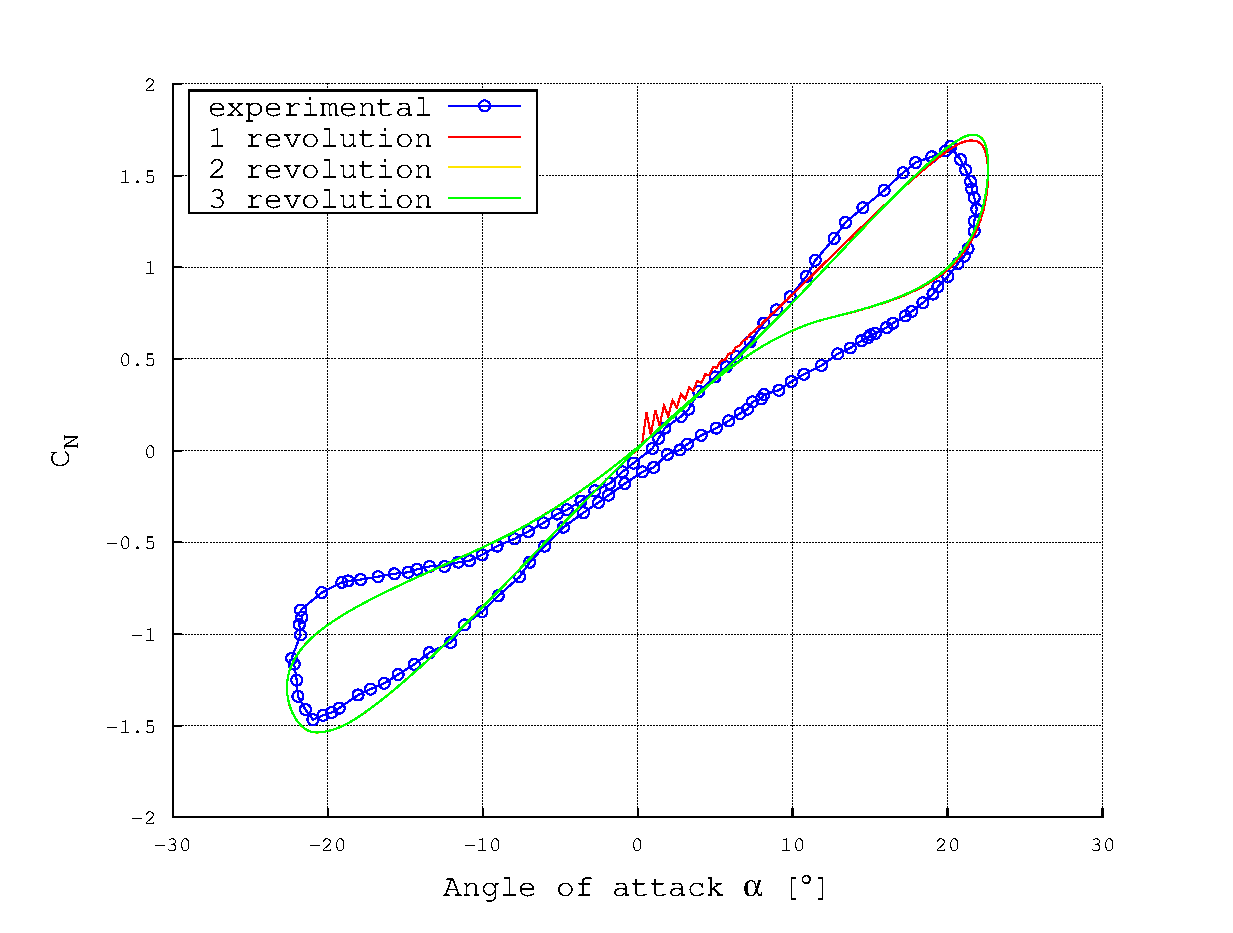
\includegraphics{CN226revolutions}}%
    \gplfronttext
  \end{picture}%
\endgroup
}
%\resizebox{\columnwidth}{!}{\input{plot}}
\end{minipage}\hspace{2pc}%
\begin{minipage}{18pc}
\resizebox{\columnwidth}{!}{% GNUPLOT: LaTeX picture with Postscript
\begingroup
  \makeatletter
  \providecommand\color[2][]{%
    \GenericError{(gnuplot) \space\space\space\@spaces}{%
      Package color not loaded in conjunction with
      terminal option `colourtext'%
    }{See the gnuplot documentation for explanation.%
    }{Either use 'blacktext' in gnuplot or load the package
      color.sty in LaTeX.}%
    \renewcommand\color[2][]{}%
  }%
  \providecommand\includegraphics[2][]{%
    \GenericError{(gnuplot) \space\space\space\@spaces}{%
      Package graphicx or graphics not loaded%
    }{See the gnuplot documentation for explanation.%
    }{The gnuplot epslatex terminal needs graphicx.sty or graphics.sty.}%
    \renewcommand\includegraphics[2][]{}%
  }%
  \providecommand\rotatebox[2]{#2}%
  \@ifundefined{ifGPcolor}{%
    \newif\ifGPcolor
    \GPcolorfalse
  }{}%
  \@ifundefined{ifGPblacktext}{%
    \newif\ifGPblacktext
    \GPblacktexttrue
  }{}%
  % define a \g@addto@macro without @ in the name:
  \let\gplgaddtomacro\g@addto@macro
  % define empty templates for all commands taking text:
  \gdef\gplbacktext{}%
  \gdef\gplfronttext{}%
  \makeatother
  \ifGPblacktext
    % no textcolor at all
    \def\colorrgb#1{}%
    \def\colorgray#1{}%
  \else
    % gray or color?
    \ifGPcolor
      \def\colorrgb#1{\color[rgb]{#1}}%
      \def\colorgray#1{\color[gray]{#1}}%
      \expandafter\def\csname LTw\endcsname{\color{white}}%
      \expandafter\def\csname LTb\endcsname{\color{black}}%
      \expandafter\def\csname LTa\endcsname{\color{black}}%
      \expandafter\def\csname LT0\endcsname{\color[rgb]{1,0,0}}%
      \expandafter\def\csname LT1\endcsname{\color[rgb]{0,1,0}}%
      \expandafter\def\csname LT2\endcsname{\color[rgb]{0,0,1}}%
      \expandafter\def\csname LT3\endcsname{\color[rgb]{1,0,1}}%
      \expandafter\def\csname LT4\endcsname{\color[rgb]{0,1,1}}%
      \expandafter\def\csname LT5\endcsname{\color[rgb]{1,1,0}}%
      \expandafter\def\csname LT6\endcsname{\color[rgb]{0,0,0}}%
      \expandafter\def\csname LT7\endcsname{\color[rgb]{1,0.3,0}}%
      \expandafter\def\csname LT8\endcsname{\color[rgb]{0.5,0.5,0.5}}%
    \else
      % gray
      \def\colorrgb#1{\color{black}}%
      \def\colorgray#1{\color[gray]{#1}}%
      \expandafter\def\csname LTw\endcsname{\color{white}}%
      \expandafter\def\csname LTb\endcsname{\color{black}}%
      \expandafter\def\csname LTa\endcsname{\color{black}}%
      \expandafter\def\csname LT0\endcsname{\color{black}}%
      \expandafter\def\csname LT1\endcsname{\color{black}}%
      \expandafter\def\csname LT2\endcsname{\color{black}}%
      \expandafter\def\csname LT3\endcsname{\color{black}}%
      \expandafter\def\csname LT4\endcsname{\color{black}}%
      \expandafter\def\csname LT5\endcsname{\color{black}}%
      \expandafter\def\csname LT6\endcsname{\color{black}}%
      \expandafter\def\csname LT7\endcsname{\color{black}}%
      \expandafter\def\csname LT8\endcsname{\color{black}}%
    \fi
  \fi
  \setlength{\unitlength}{0.0500bp}%
  \begin{picture}(7200.00,5040.00)%
    \gplgaddtomacro\gplbacktext{%
      \csname LTb\endcsname%
      \put(1078,704){\makebox(0,0)[r]{\strut{}-0.05}}%
      \csname LTb\endcsname%
      \put(1078,1074){\makebox(0,0)[r]{\strut{} 0}}%
      \csname LTb\endcsname%
      \put(1078,1444){\makebox(0,0)[r]{\strut{} 0.05}}%
      \csname LTb\endcsname%
      \put(1078,1814){\makebox(0,0)[r]{\strut{} 0.1}}%
      \csname LTb\endcsname%
      \put(1078,2184){\makebox(0,0)[r]{\strut{} 0.15}}%
      \csname LTb\endcsname%
      \put(1078,2554){\makebox(0,0)[r]{\strut{} 0.2}}%
      \csname LTb\endcsname%
      \put(1078,2925){\makebox(0,0)[r]{\strut{} 0.25}}%
      \csname LTb\endcsname%
      \put(1078,3295){\makebox(0,0)[r]{\strut{} 0.3}}%
      \csname LTb\endcsname%
      \put(1078,3665){\makebox(0,0)[r]{\strut{} 0.35}}%
      \csname LTb\endcsname%
      \put(1078,4035){\makebox(0,0)[r]{\strut{} 0.4}}%
      \csname LTb\endcsname%
      \put(1078,4405){\makebox(0,0)[r]{\strut{} 0.45}}%
      \csname LTb\endcsname%
      \put(1078,4775){\makebox(0,0)[r]{\strut{} 0.5}}%
      \csname LTb\endcsname%
      \put(1210,484){\makebox(0,0){\strut{}-25}}%
      \csname LTb\endcsname%
      \put(1769,484){\makebox(0,0){\strut{}-20}}%
      \csname LTb\endcsname%
      \put(2329,484){\makebox(0,0){\strut{}-15}}%
      \csname LTb\endcsname%
      \put(2888,484){\makebox(0,0){\strut{}-10}}%
      \csname LTb\endcsname%
      \put(3447,484){\makebox(0,0){\strut{}-5}}%
      \csname LTb\endcsname%
      \put(4007,484){\makebox(0,0){\strut{} 0}}%
      \csname LTb\endcsname%
      \put(4566,484){\makebox(0,0){\strut{} 5}}%
      \csname LTb\endcsname%
      \put(5125,484){\makebox(0,0){\strut{} 10}}%
      \csname LTb\endcsname%
      \put(5684,484){\makebox(0,0){\strut{} 15}}%
      \csname LTb\endcsname%
      \put(6244,484){\makebox(0,0){\strut{} 20}}%
      \csname LTb\endcsname%
      \put(6803,484){\makebox(0,0){\strut{} 25}}%
      \put(176,2739){\rotatebox{-270}{\makebox(0,0){\strut{}$C_T$}}}%
      \put(4006,154){\makebox(0,0){\strut{}Angle of attack {$\alpha$} [$\degree$]}}%
    }%
    \gplgaddtomacro\gplfronttext{%
      \csname LTb\endcsname%
      \put(4371,4602){\makebox(0,0)[r]{\strut{}experimental}}%
      \csname LTb\endcsname%
      \put(4371,4382){\makebox(0,0)[r]{\strut{}1 revolution}}%
      \csname LTb\endcsname%
      \put(4371,4162){\makebox(0,0)[r]{\strut{}2 revolution}}%
      \csname LTb\endcsname%
      \put(4371,3942){\makebox(0,0)[r]{\strut{}3 revolution}}%
    }%
    \gplbacktext
    \put(0,0){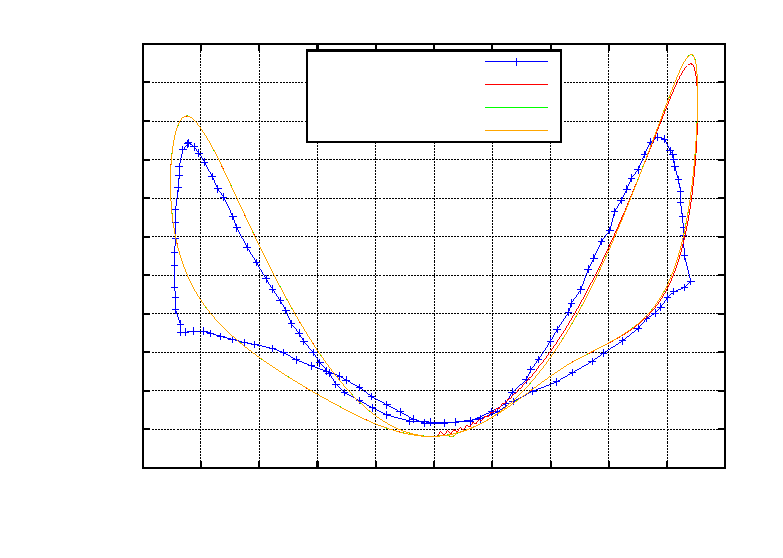
\includegraphics{CT226revolutions}}%
    \gplfronttext
  \end{picture}%
\endgroup
}
\end{minipage}
\caption{\label{revolutions}Normal (left) and tangential (right) force coefficients varying the number of revolutions for a pitching motion of NACA0021 airfoil with a maximum amplitude of 22.6$\degree$.}
\end{figure}

\textbf{Spatial sensitivity:} A test of the response of the model
to the variation in the size of the mesh is carried out. A mesh of approximatively 1e5 of cells with a local refinement around the blade is used as a reference mesh (Figure \ref{figrefmesh}), this topology is kept constant and globally refinement are applied for this study; it means the mesh is proportionally scaled in every coordinates.

\begin{figure}[h]
\begin{minipage}{36pc}
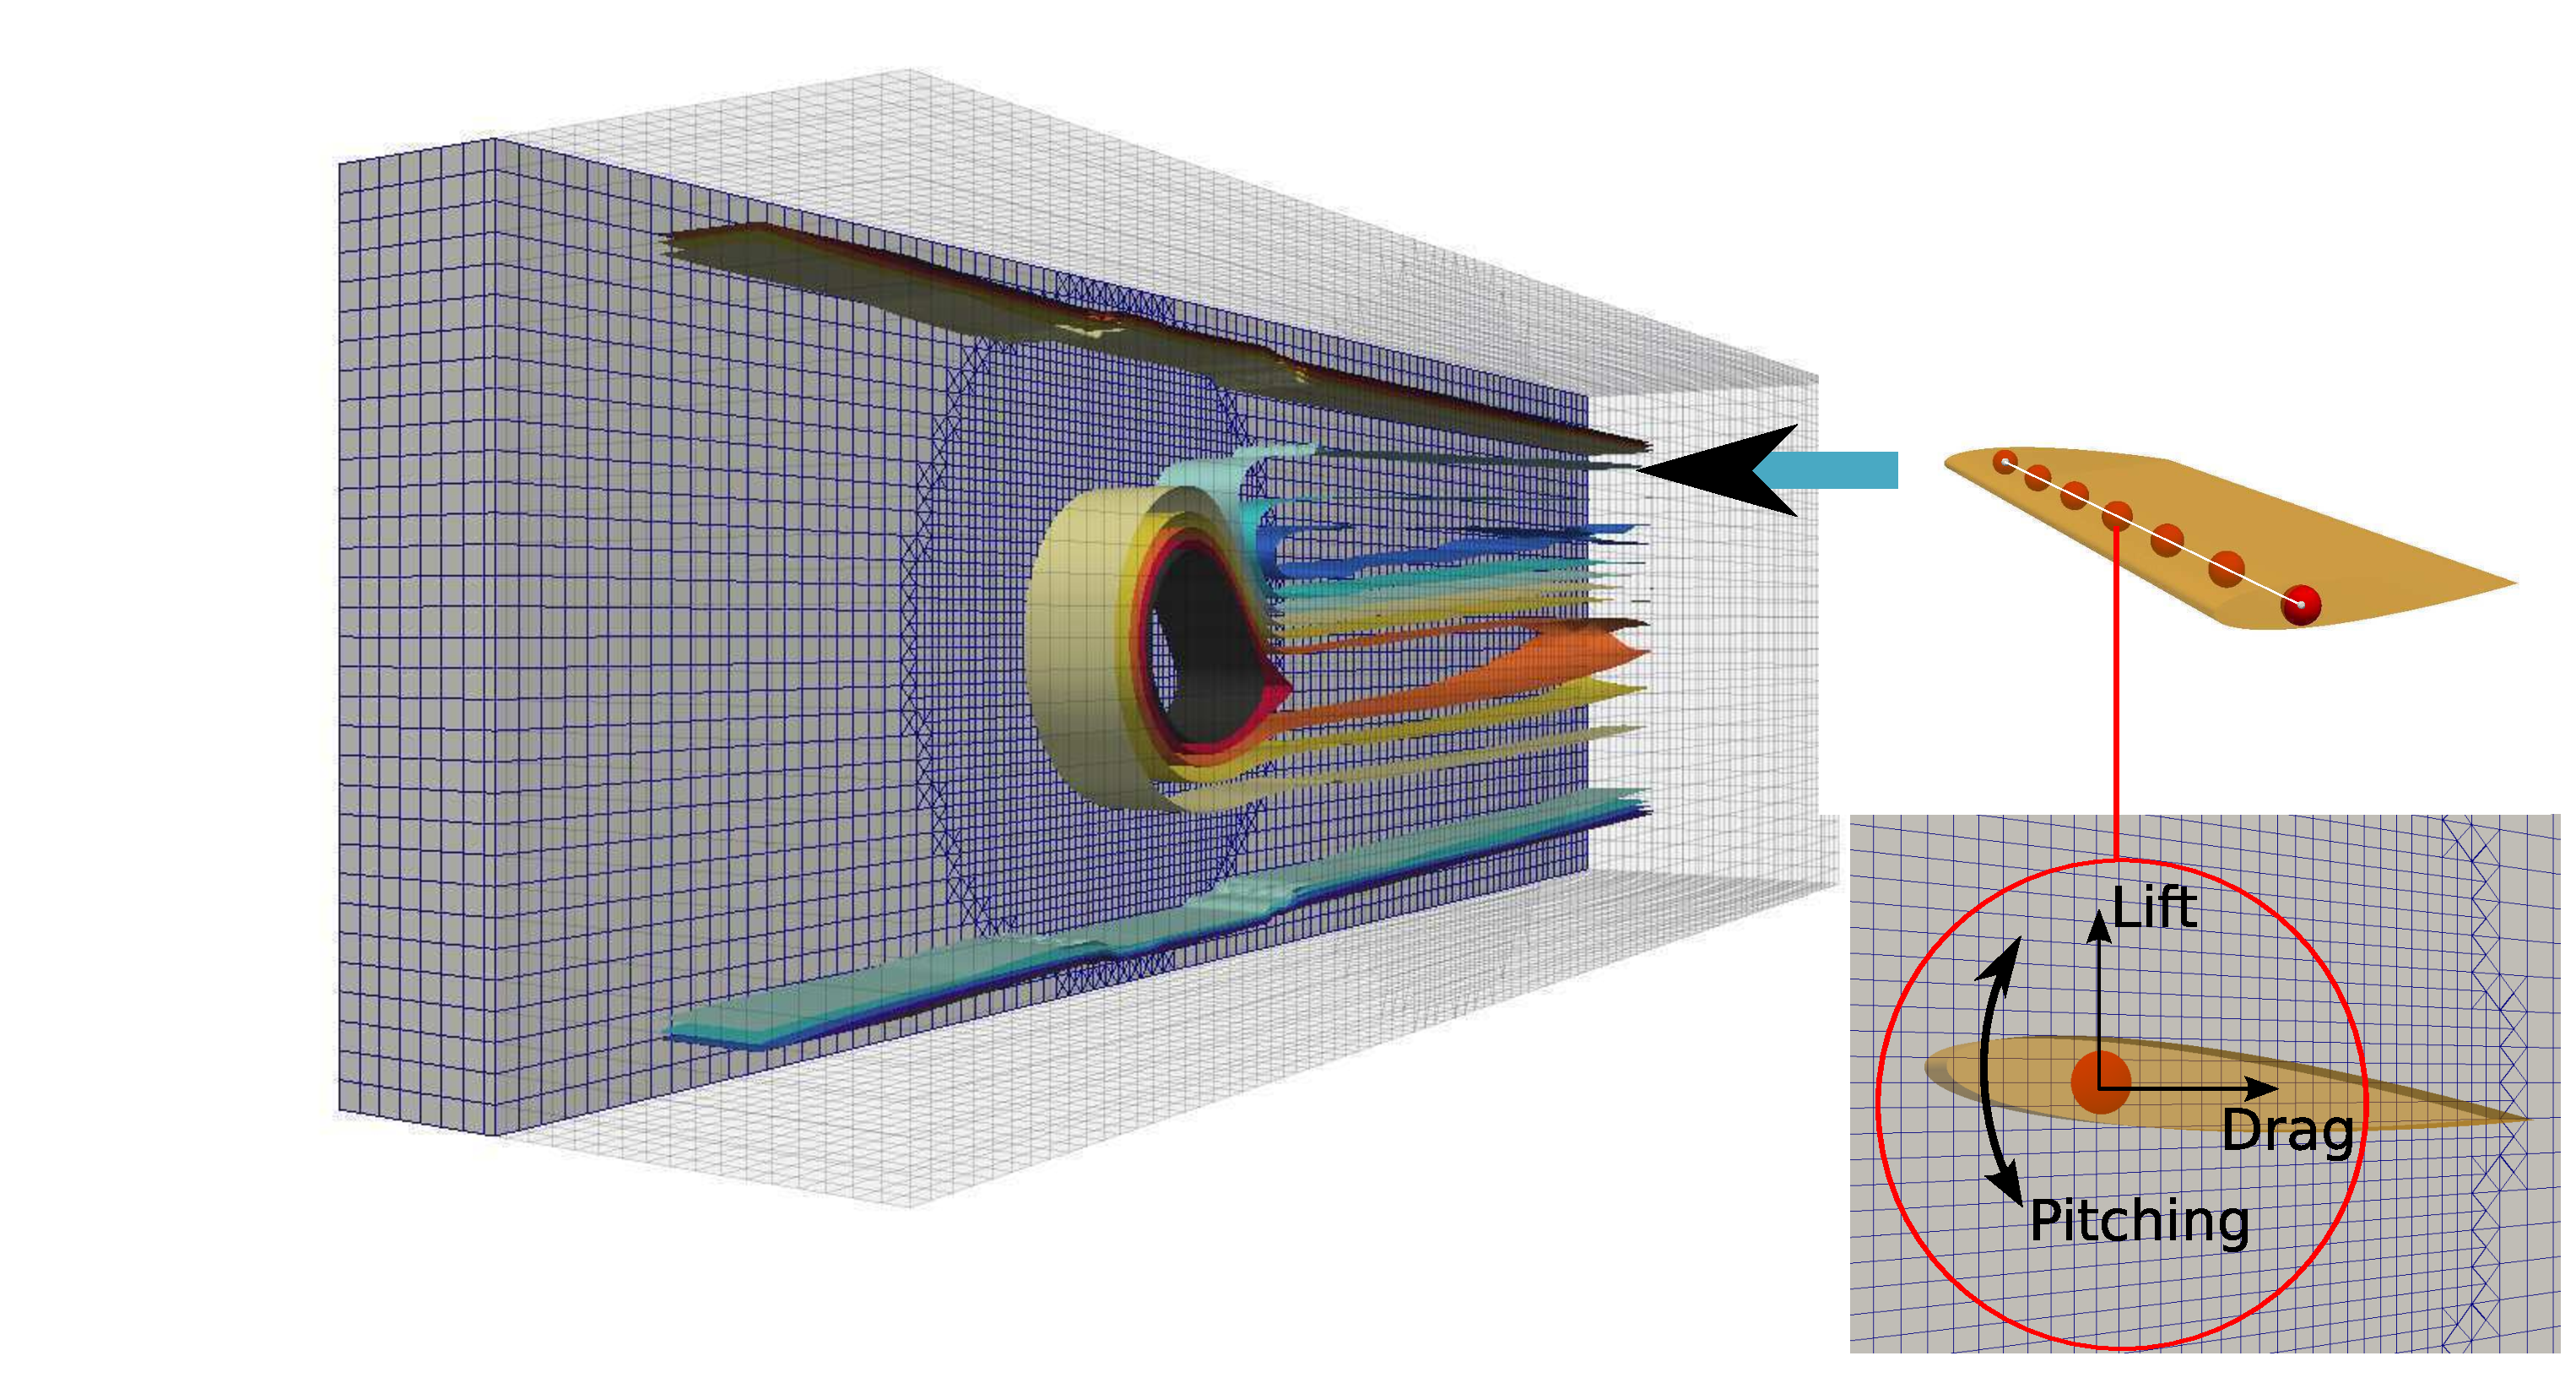
\includegraphics[width=0.5\columnwidth]{vorticityZ2.eps}
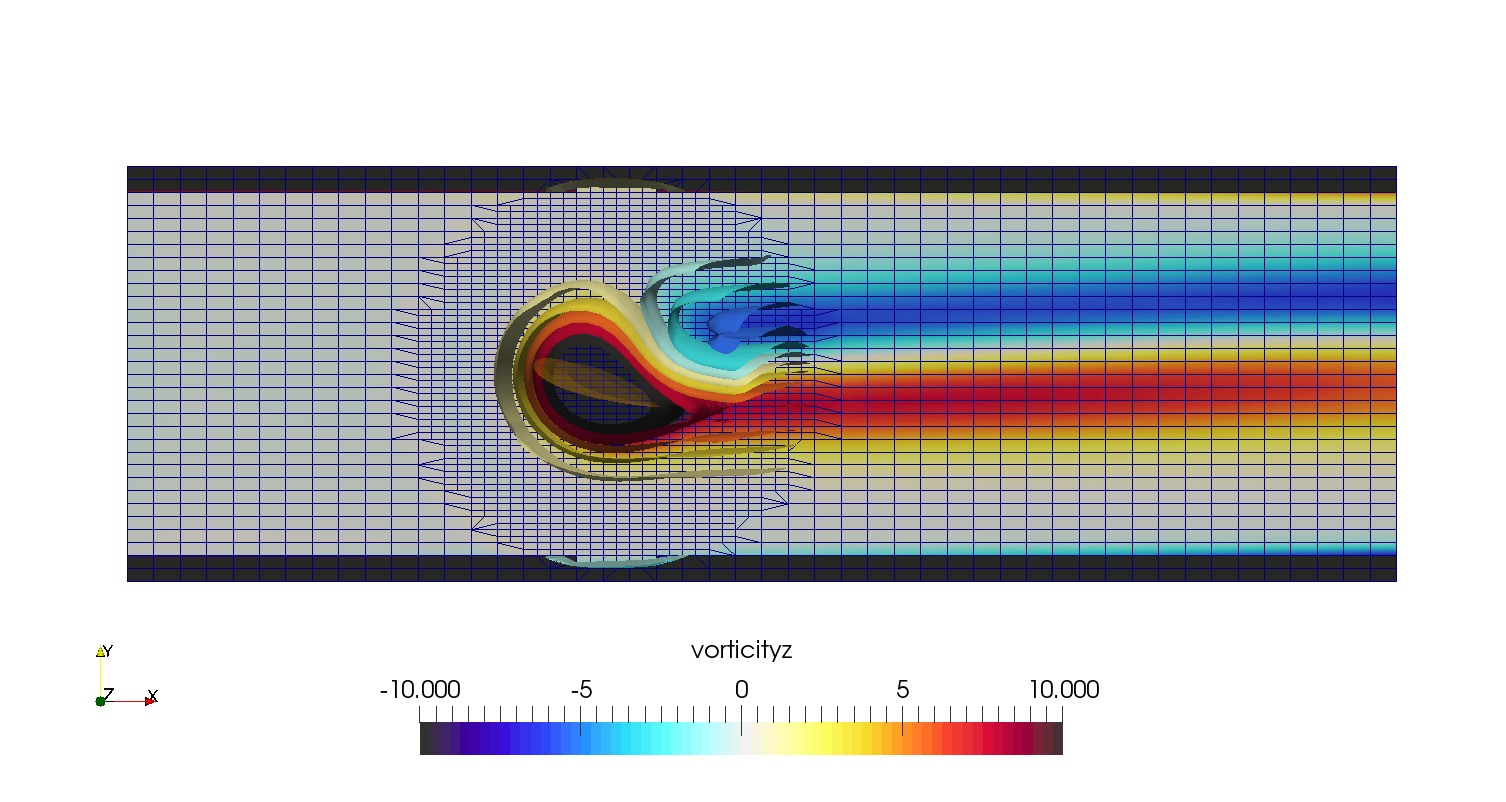
\includegraphics[width=0.5\columnwidth]{vorticityZ.png}
%\resizebox{\columnwidth}{!}{\input{plot}}
\end{minipage}%
\caption{\label{figrefmesh} Illustration of a reference mesh section and vorticity isosurfaces generated by the pitching motion around the blade.}
\end{figure}

From Figure \ref{figmesh}, it could be noticed that there is a  variation in the results either for a decreasing or increasing in the mesh resolution. Between the refinement of 150 and 200\% not considerable changes are obtained in the results, so a major refinement is not justified due this will not give any possible improvement in the accuracy of the results.

\begin{figure}[h]
\begin{minipage}{18pc}
\resizebox{\columnwidth}{!}{% GNUPLOT: LaTeX picture with Postscript
\begingroup
  \makeatletter
  \providecommand\color[2][]{%
    \GenericError{(gnuplot) \space\space\space\@spaces}{%
      Package color not loaded in conjunction with
      terminal option `colourtext'%
    }{See the gnuplot documentation for explanation.%
    }{Either use 'blacktext' in gnuplot or load the package
      color.sty in LaTeX.}%
    \renewcommand\color[2][]{}%
  }%
  \providecommand\includegraphics[2][]{%
    \GenericError{(gnuplot) \space\space\space\@spaces}{%
      Package graphicx or graphics not loaded%
    }{See the gnuplot documentation for explanation.%
    }{The gnuplot epslatex terminal needs graphicx.sty or graphics.sty.}%
    \renewcommand\includegraphics[2][]{}%
  }%
  \providecommand\rotatebox[2]{#2}%
  \@ifundefined{ifGPcolor}{%
    \newif\ifGPcolor
    \GPcolorfalse
  }{}%
  \@ifundefined{ifGPblacktext}{%
    \newif\ifGPblacktext
    \GPblacktexttrue
  }{}%
  % define a \g@addto@macro without @ in the name:
  \let\gplgaddtomacro\g@addto@macro
  % define empty templates for all commands taking text:
  \gdef\gplbacktext{}%
  \gdef\gplfronttext{}%
  \makeatother
  \ifGPblacktext
    % no textcolor at all
    \def\colorrgb#1{}%
    \def\colorgray#1{}%
  \else
    % gray or color?
    \ifGPcolor
      \def\colorrgb#1{\color[rgb]{#1}}%
      \def\colorgray#1{\color[gray]{#1}}%
      \expandafter\def\csname LTw\endcsname{\color{white}}%
      \expandafter\def\csname LTb\endcsname{\color{black}}%
      \expandafter\def\csname LTa\endcsname{\color{black}}%
      \expandafter\def\csname LT0\endcsname{\color[rgb]{1,0,0}}%
      \expandafter\def\csname LT1\endcsname{\color[rgb]{0,1,0}}%
      \expandafter\def\csname LT2\endcsname{\color[rgb]{0,0,1}}%
      \expandafter\def\csname LT3\endcsname{\color[rgb]{1,0,1}}%
      \expandafter\def\csname LT4\endcsname{\color[rgb]{0,1,1}}%
      \expandafter\def\csname LT5\endcsname{\color[rgb]{1,1,0}}%
      \expandafter\def\csname LT6\endcsname{\color[rgb]{0,0,0}}%
      \expandafter\def\csname LT7\endcsname{\color[rgb]{1,0.3,0}}%
      \expandafter\def\csname LT8\endcsname{\color[rgb]{0.5,0.5,0.5}}%
    \else
      % gray
      \def\colorrgb#1{\color{black}}%
      \def\colorgray#1{\color[gray]{#1}}%
      \expandafter\def\csname LTw\endcsname{\color{white}}%
      \expandafter\def\csname LTb\endcsname{\color{black}}%
      \expandafter\def\csname LTa\endcsname{\color{black}}%
      \expandafter\def\csname LT0\endcsname{\color{black}}%
      \expandafter\def\csname LT1\endcsname{\color{black}}%
      \expandafter\def\csname LT2\endcsname{\color{black}}%
      \expandafter\def\csname LT3\endcsname{\color{black}}%
      \expandafter\def\csname LT4\endcsname{\color{black}}%
      \expandafter\def\csname LT5\endcsname{\color{black}}%
      \expandafter\def\csname LT6\endcsname{\color{black}}%
      \expandafter\def\csname LT7\endcsname{\color{black}}%
      \expandafter\def\csname LT8\endcsname{\color{black}}%
    \fi
  \fi
  \setlength{\unitlength}{0.0500bp}%
  \begin{picture}(7200.00,5040.00)%
    \gplgaddtomacro\gplbacktext{%
      \csname LTb\endcsname%
      \put(946,704){\makebox(0,0)[r]{\strut{}-2}}%
      \csname LTb\endcsname%
      \put(946,1213){\makebox(0,0)[r]{\strut{}-1.5}}%
      \csname LTb\endcsname%
      \put(946,1722){\makebox(0,0)[r]{\strut{}-1}}%
      \csname LTb\endcsname%
      \put(946,2231){\makebox(0,0)[r]{\strut{}-0.5}}%
      \csname LTb\endcsname%
      \put(946,2740){\makebox(0,0)[r]{\strut{} 0}}%
      \csname LTb\endcsname%
      \put(946,3248){\makebox(0,0)[r]{\strut{} 0.5}}%
      \csname LTb\endcsname%
      \put(946,3757){\makebox(0,0)[r]{\strut{} 1}}%
      \csname LTb\endcsname%
      \put(946,4266){\makebox(0,0)[r]{\strut{} 1.5}}%
      \csname LTb\endcsname%
      \put(946,4775){\makebox(0,0)[r]{\strut{} 2}}%
      \csname LTb\endcsname%
      \put(1078,484){\makebox(0,0){\strut{}-25}}%
      \csname LTb\endcsname%
      \put(1651,484){\makebox(0,0){\strut{}-20}}%
      \csname LTb\endcsname%
      \put(2223,484){\makebox(0,0){\strut{}-15}}%
      \csname LTb\endcsname%
      \put(2796,484){\makebox(0,0){\strut{}-10}}%
      \csname LTb\endcsname%
      \put(3368,484){\makebox(0,0){\strut{}-5}}%
      \csname LTb\endcsname%
      \put(3941,484){\makebox(0,0){\strut{} 0}}%
      \csname LTb\endcsname%
      \put(4513,484){\makebox(0,0){\strut{} 5}}%
      \csname LTb\endcsname%
      \put(5086,484){\makebox(0,0){\strut{} 10}}%
      \csname LTb\endcsname%
      \put(5658,484){\makebox(0,0){\strut{} 15}}%
      \csname LTb\endcsname%
      \put(6231,484){\makebox(0,0){\strut{} 20}}%
      \csname LTb\endcsname%
      \put(6803,484){\makebox(0,0){\strut{} 25}}%
      \put(176,2739){\rotatebox{-270}{\makebox(0,0){\strut{}$C_N$}}}%
      \put(3940,154){\makebox(0,0){\strut{}Angle of attack {$\alpha$} [$\degree$]}}%
    }%
    \gplgaddtomacro\gplfronttext{%
      \csname LTb\endcsname%
      \put(3322,4602){\makebox(0,0)[r]{\strut{}experimental}}%
      \csname LTb\endcsname%
      \put(3322,4382){\makebox(0,0)[r]{\strut{}reference mesh}}%
      \csname LTb\endcsname%
      \put(3322,4162){\makebox(0,0)[r]{\strut{}50$\%$ refinement}}%
      \csname LTb\endcsname%
      \put(3322,3942){\makebox(0,0)[r]{\strut{}150$\%$ refinement}}%
      \csname LTb\endcsname%
      \put(3322,3722){\makebox(0,0)[r]{\strut{}200$\%$ refinement}}%
    }%
    \gplbacktext
    \put(0,0){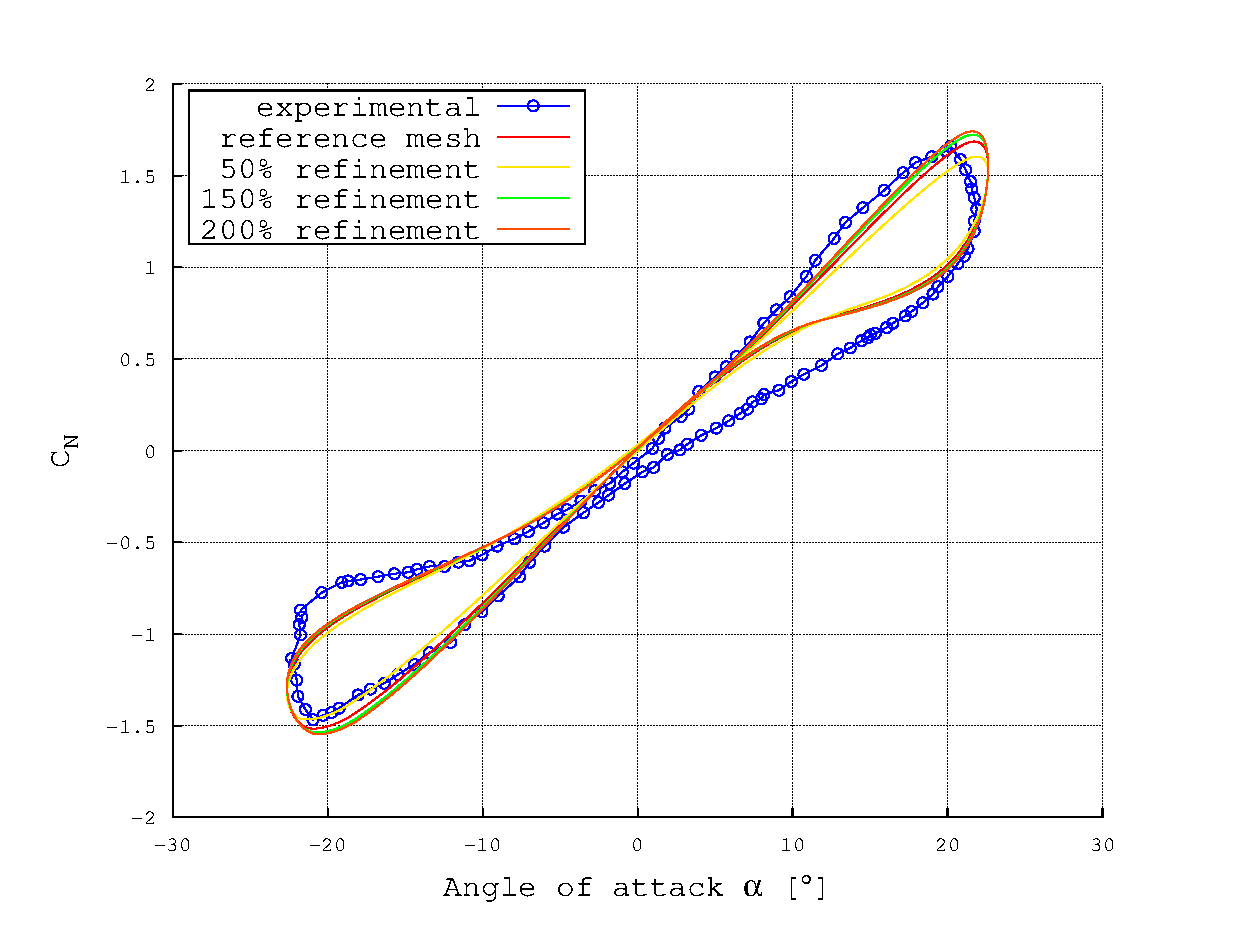
\includegraphics{CNmesh}}%
    \gplfronttext
  \end{picture}%
\endgroup
}
%\resizebox{\columnwidth}{!}{\input{plot}}
\end{minipage}\hspace{2pc}%
\begin{minipage}{18pc}
\resizebox{\columnwidth}{!}{% GNUPLOT: LaTeX picture with Postscript
\begingroup
  \makeatletter
  \providecommand\color[2][]{%
    \GenericError{(gnuplot) \space\space\space\@spaces}{%
      Package color not loaded in conjunction with
      terminal option `colourtext'%
    }{See the gnuplot documentation for explanation.%
    }{Either use 'blacktext' in gnuplot or load the package
      color.sty in LaTeX.}%
    \renewcommand\color[2][]{}%
  }%
  \providecommand\includegraphics[2][]{%
    \GenericError{(gnuplot) \space\space\space\@spaces}{%
      Package graphicx or graphics not loaded%
    }{See the gnuplot documentation for explanation.%
    }{The gnuplot epslatex terminal needs graphicx.sty or graphics.sty.}%
    \renewcommand\includegraphics[2][]{}%
  }%
  \providecommand\rotatebox[2]{#2}%
  \@ifundefined{ifGPcolor}{%
    \newif\ifGPcolor
    \GPcolorfalse
  }{}%
  \@ifundefined{ifGPblacktext}{%
    \newif\ifGPblacktext
    \GPblacktexttrue
  }{}%
  % define a \g@addto@macro without @ in the name:
  \let\gplgaddtomacro\g@addto@macro
  % define empty templates for all commands taking text:
  \gdef\gplbacktext{}%
  \gdef\gplfronttext{}%
  \makeatother
  \ifGPblacktext
    % no textcolor at all
    \def\colorrgb#1{}%
    \def\colorgray#1{}%
  \else
    % gray or color?
    \ifGPcolor
      \def\colorrgb#1{\color[rgb]{#1}}%
      \def\colorgray#1{\color[gray]{#1}}%
      \expandafter\def\csname LTw\endcsname{\color{white}}%
      \expandafter\def\csname LTb\endcsname{\color{black}}%
      \expandafter\def\csname LTa\endcsname{\color{black}}%
      \expandafter\def\csname LT0\endcsname{\color[rgb]{1,0,0}}%
      \expandafter\def\csname LT1\endcsname{\color[rgb]{0,1,0}}%
      \expandafter\def\csname LT2\endcsname{\color[rgb]{0,0,1}}%
      \expandafter\def\csname LT3\endcsname{\color[rgb]{1,0,1}}%
      \expandafter\def\csname LT4\endcsname{\color[rgb]{0,1,1}}%
      \expandafter\def\csname LT5\endcsname{\color[rgb]{1,1,0}}%
      \expandafter\def\csname LT6\endcsname{\color[rgb]{0,0,0}}%
      \expandafter\def\csname LT7\endcsname{\color[rgb]{1,0.3,0}}%
      \expandafter\def\csname LT8\endcsname{\color[rgb]{0.5,0.5,0.5}}%
    \else
      % gray
      \def\colorrgb#1{\color{black}}%
      \def\colorgray#1{\color[gray]{#1}}%
      \expandafter\def\csname LTw\endcsname{\color{white}}%
      \expandafter\def\csname LTb\endcsname{\color{black}}%
      \expandafter\def\csname LTa\endcsname{\color{black}}%
      \expandafter\def\csname LT0\endcsname{\color{black}}%
      \expandafter\def\csname LT1\endcsname{\color{black}}%
      \expandafter\def\csname LT2\endcsname{\color{black}}%
      \expandafter\def\csname LT3\endcsname{\color{black}}%
      \expandafter\def\csname LT4\endcsname{\color{black}}%
      \expandafter\def\csname LT5\endcsname{\color{black}}%
      \expandafter\def\csname LT6\endcsname{\color{black}}%
      \expandafter\def\csname LT7\endcsname{\color{black}}%
      \expandafter\def\csname LT8\endcsname{\color{black}}%
    \fi
  \fi
  \setlength{\unitlength}{0.0500bp}%
  \begin{picture}(7200.00,5040.00)%
    \gplgaddtomacro\gplbacktext{%
      \csname LTb\endcsname%
      \put(1078,704){\makebox(0,0)[r]{\strut{}-0.05}}%
      \csname LTb\endcsname%
      \put(1078,1074){\makebox(0,0)[r]{\strut{} 0}}%
      \csname LTb\endcsname%
      \put(1078,1444){\makebox(0,0)[r]{\strut{} 0.05}}%
      \csname LTb\endcsname%
      \put(1078,1814){\makebox(0,0)[r]{\strut{} 0.1}}%
      \csname LTb\endcsname%
      \put(1078,2184){\makebox(0,0)[r]{\strut{} 0.15}}%
      \csname LTb\endcsname%
      \put(1078,2554){\makebox(0,0)[r]{\strut{} 0.2}}%
      \csname LTb\endcsname%
      \put(1078,2925){\makebox(0,0)[r]{\strut{} 0.25}}%
      \csname LTb\endcsname%
      \put(1078,3295){\makebox(0,0)[r]{\strut{} 0.3}}%
      \csname LTb\endcsname%
      \put(1078,3665){\makebox(0,0)[r]{\strut{} 0.35}}%
      \csname LTb\endcsname%
      \put(1078,4035){\makebox(0,0)[r]{\strut{} 0.4}}%
      \csname LTb\endcsname%
      \put(1078,4405){\makebox(0,0)[r]{\strut{} 0.45}}%
      \csname LTb\endcsname%
      \put(1078,4775){\makebox(0,0)[r]{\strut{} 0.5}}%
      \csname LTb\endcsname%
      \put(1210,484){\makebox(0,0){\strut{}-25}}%
      \csname LTb\endcsname%
      \put(1769,484){\makebox(0,0){\strut{}-20}}%
      \csname LTb\endcsname%
      \put(2329,484){\makebox(0,0){\strut{}-15}}%
      \csname LTb\endcsname%
      \put(2888,484){\makebox(0,0){\strut{}-10}}%
      \csname LTb\endcsname%
      \put(3447,484){\makebox(0,0){\strut{}-5}}%
      \csname LTb\endcsname%
      \put(4007,484){\makebox(0,0){\strut{} 0}}%
      \csname LTb\endcsname%
      \put(4566,484){\makebox(0,0){\strut{} 5}}%
      \csname LTb\endcsname%
      \put(5125,484){\makebox(0,0){\strut{} 10}}%
      \csname LTb\endcsname%
      \put(5684,484){\makebox(0,0){\strut{} 15}}%
      \csname LTb\endcsname%
      \put(6244,484){\makebox(0,0){\strut{} 20}}%
      \csname LTb\endcsname%
      \put(6803,484){\makebox(0,0){\strut{} 25}}%
      \put(176,2739){\rotatebox{-270}{\makebox(0,0){\strut{}$C_T$}}}%
      \put(4006,154){\makebox(0,0){\strut{}Angle of attack {$\alpha$} [$\degree$]}}%
    }%
    \gplgaddtomacro\gplfronttext{%
      \csname LTb\endcsname%
      \put(4635,4602){\makebox(0,0)[r]{\strut{}experimental}}%
      \csname LTb\endcsname%
      \put(4635,4382){\makebox(0,0)[r]{\strut{}reference mesh}}%
      \csname LTb\endcsname%
      \put(4635,4162){\makebox(0,0)[r]{\strut{}50$\%$ refinement}}%
      \csname LTb\endcsname%
      \put(4635,3942){\makebox(0,0)[r]{\strut{}150$\%$ refinement}}%
      \csname LTb\endcsname%
      \put(4635,3722){\makebox(0,0)[r]{\strut{}200$\%$ refinement}}%
    }%
    \gplbacktext
    \put(0,0){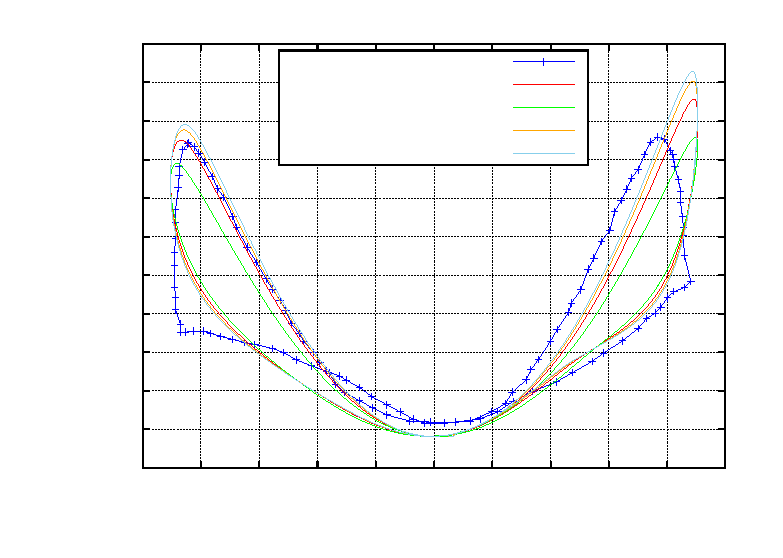
\includegraphics{CTmesh}}%
    \gplfronttext
  \end{picture}%
\endgroup
}
\end{minipage}
\caption{\label{figmesh}Normal (left) and tangential (right) force coefficients varying the size of the reference mesh for a pitching motion with a maximum amplitude of 22.6\degree\ }
\end{figure}

\textbf{Temporal sensitivity:} Different time-steps were chosen for a varying temporal discretization test, which $\Delta t$ values are 0.001, 0.003, 0.0055 and 0.0075 [s], and these correspond to around 1200, 400, 220 and 160 time-steps per revolution respectively. In this study a coarse mesh with a refinement of 25\%, compared to the reference one, was used. Results are shown in Figure \ref{figdtcoarse}.

The model is more sensitive to the spatial discretization than the temporal one;
same characteristic was obtained by Bachant et al. in
\cite{Bachant2016-VAT-ALM}. Accuracy and stability were not affected even for
big values for $\Delta t$, as long they are within the limit given by the CFL
condition; a Courant number of less than unity is required. On the other hand,
it should be considered that small time-step of discretization could cause
numerical instabilities due to the fluctuation of the flow fields resolving the
transient term $\frac{\partial \alpha}{\partial t}$.

\begin{figure}[h]
\begin{minipage}{18pc}
\resizebox{\columnwidth}{!}{% GNUPLOT: LaTeX picture with Postscript
\begingroup
  \makeatletter
  \providecommand\color[2][]{%
    \GenericError{(gnuplot) \space\space\space\@spaces}{%
      Package color not loaded in conjunction with
      terminal option `colourtext'%
    }{See the gnuplot documentation for explanation.%
    }{Either use 'blacktext' in gnuplot or load the package
      color.sty in LaTeX.}%
    \renewcommand\color[2][]{}%
  }%
  \providecommand\includegraphics[2][]{%
    \GenericError{(gnuplot) \space\space\space\@spaces}{%
      Package graphicx or graphics not loaded%
    }{See the gnuplot documentation for explanation.%
    }{The gnuplot epslatex terminal needs graphicx.sty or graphics.sty.}%
    \renewcommand\includegraphics[2][]{}%
  }%
  \providecommand\rotatebox[2]{#2}%
  \@ifundefined{ifGPcolor}{%
    \newif\ifGPcolor
    \GPcolorfalse
  }{}%
  \@ifundefined{ifGPblacktext}{%
    \newif\ifGPblacktext
    \GPblacktexttrue
  }{}%
  % define a \g@addto@macro without @ in the name:
  \let\gplgaddtomacro\g@addto@macro
  % define empty templates for all commands taking text:
  \gdef\gplbacktext{}%
  \gdef\gplfronttext{}%
  \makeatother
  \ifGPblacktext
    % no textcolor at all
    \def\colorrgb#1{}%
    \def\colorgray#1{}%
  \else
    % gray or color?
    \ifGPcolor
      \def\colorrgb#1{\color[rgb]{#1}}%
      \def\colorgray#1{\color[gray]{#1}}%
      \expandafter\def\csname LTw\endcsname{\color{white}}%
      \expandafter\def\csname LTb\endcsname{\color{black}}%
      \expandafter\def\csname LTa\endcsname{\color{black}}%
      \expandafter\def\csname LT0\endcsname{\color[rgb]{1,0,0}}%
      \expandafter\def\csname LT1\endcsname{\color[rgb]{0,1,0}}%
      \expandafter\def\csname LT2\endcsname{\color[rgb]{0,0,1}}%
      \expandafter\def\csname LT3\endcsname{\color[rgb]{1,0,1}}%
      \expandafter\def\csname LT4\endcsname{\color[rgb]{0,1,1}}%
      \expandafter\def\csname LT5\endcsname{\color[rgb]{1,1,0}}%
      \expandafter\def\csname LT6\endcsname{\color[rgb]{0,0,0}}%
      \expandafter\def\csname LT7\endcsname{\color[rgb]{1,0.3,0}}%
      \expandafter\def\csname LT8\endcsname{\color[rgb]{0.5,0.5,0.5}}%
    \else
      % gray
      \def\colorrgb#1{\color{black}}%
      \def\colorgray#1{\color[gray]{#1}}%
      \expandafter\def\csname LTw\endcsname{\color{white}}%
      \expandafter\def\csname LTb\endcsname{\color{black}}%
      \expandafter\def\csname LTa\endcsname{\color{black}}%
      \expandafter\def\csname LT0\endcsname{\color{black}}%
      \expandafter\def\csname LT1\endcsname{\color{black}}%
      \expandafter\def\csname LT2\endcsname{\color{black}}%
      \expandafter\def\csname LT3\endcsname{\color{black}}%
      \expandafter\def\csname LT4\endcsname{\color{black}}%
      \expandafter\def\csname LT5\endcsname{\color{black}}%
      \expandafter\def\csname LT6\endcsname{\color{black}}%
      \expandafter\def\csname LT7\endcsname{\color{black}}%
      \expandafter\def\csname LT8\endcsname{\color{black}}%
    \fi
  \fi
  \setlength{\unitlength}{0.0500bp}%
  \begin{picture}(7200.00,5040.00)%
    \gplgaddtomacro\gplbacktext{%
      \csname LTb\endcsname%
      \put(946,704){\makebox(0,0)[r]{\strut{}-2}}%
      \csname LTb\endcsname%
      \put(946,1213){\makebox(0,0)[r]{\strut{}-1.5}}%
      \csname LTb\endcsname%
      \put(946,1722){\makebox(0,0)[r]{\strut{}-1}}%
      \csname LTb\endcsname%
      \put(946,2231){\makebox(0,0)[r]{\strut{}-0.5}}%
      \csname LTb\endcsname%
      \put(946,2740){\makebox(0,0)[r]{\strut{} 0}}%
      \csname LTb\endcsname%
      \put(946,3248){\makebox(0,0)[r]{\strut{} 0.5}}%
      \csname LTb\endcsname%
      \put(946,3757){\makebox(0,0)[r]{\strut{} 1}}%
      \csname LTb\endcsname%
      \put(946,4266){\makebox(0,0)[r]{\strut{} 1.5}}%
      \csname LTb\endcsname%
      \put(946,4775){\makebox(0,0)[r]{\strut{} 2}}%
      \csname LTb\endcsname%
      \put(1078,484){\makebox(0,0){\strut{}-25}}%
      \csname LTb\endcsname%
      \put(1651,484){\makebox(0,0){\strut{}-20}}%
      \csname LTb\endcsname%
      \put(2223,484){\makebox(0,0){\strut{}-15}}%
      \csname LTb\endcsname%
      \put(2796,484){\makebox(0,0){\strut{}-10}}%
      \csname LTb\endcsname%
      \put(3368,484){\makebox(0,0){\strut{}-5}}%
      \csname LTb\endcsname%
      \put(3941,484){\makebox(0,0){\strut{} 0}}%
      \csname LTb\endcsname%
      \put(4513,484){\makebox(0,0){\strut{} 5}}%
      \csname LTb\endcsname%
      \put(5086,484){\makebox(0,0){\strut{} 10}}%
      \csname LTb\endcsname%
      \put(5658,484){\makebox(0,0){\strut{} 15}}%
      \csname LTb\endcsname%
      \put(6231,484){\makebox(0,0){\strut{} 20}}%
      \csname LTb\endcsname%
      \put(6803,484){\makebox(0,0){\strut{} 25}}%
      \put(176,2739){\rotatebox{-270}{\makebox(0,0){\strut{}$C_N$}}}%
      \put(3940,154){\makebox(0,0){\strut{}Angle of attack {$\alpha$} [$\degree$]}}%
    }%
    \gplgaddtomacro\gplfronttext{%
      \csname LTb\endcsname%
      \put(2794,4602){\makebox(0,0)[r]{\strut{}experimental}}%
      \csname LTb\endcsname%
      \put(2794,4382){\makebox(0,0)[r]{\strut{}$\Delta$t=0.001[s]}}%
      \csname LTb\endcsname%
      \put(2794,4162){\makebox(0,0)[r]{\strut{}$\Delta$t=0.003[s]}}%
      \csname LTb\endcsname%
      \put(2794,3942){\makebox(0,0)[r]{\strut{}$\Delta$t=0.0055[s]}}%
      \csname LTb\endcsname%
      \put(2794,3722){\makebox(0,0)[r]{\strut{}$\Delta$t=0.0075[s]}}%
    }%
    \gplbacktext
    \put(0,0){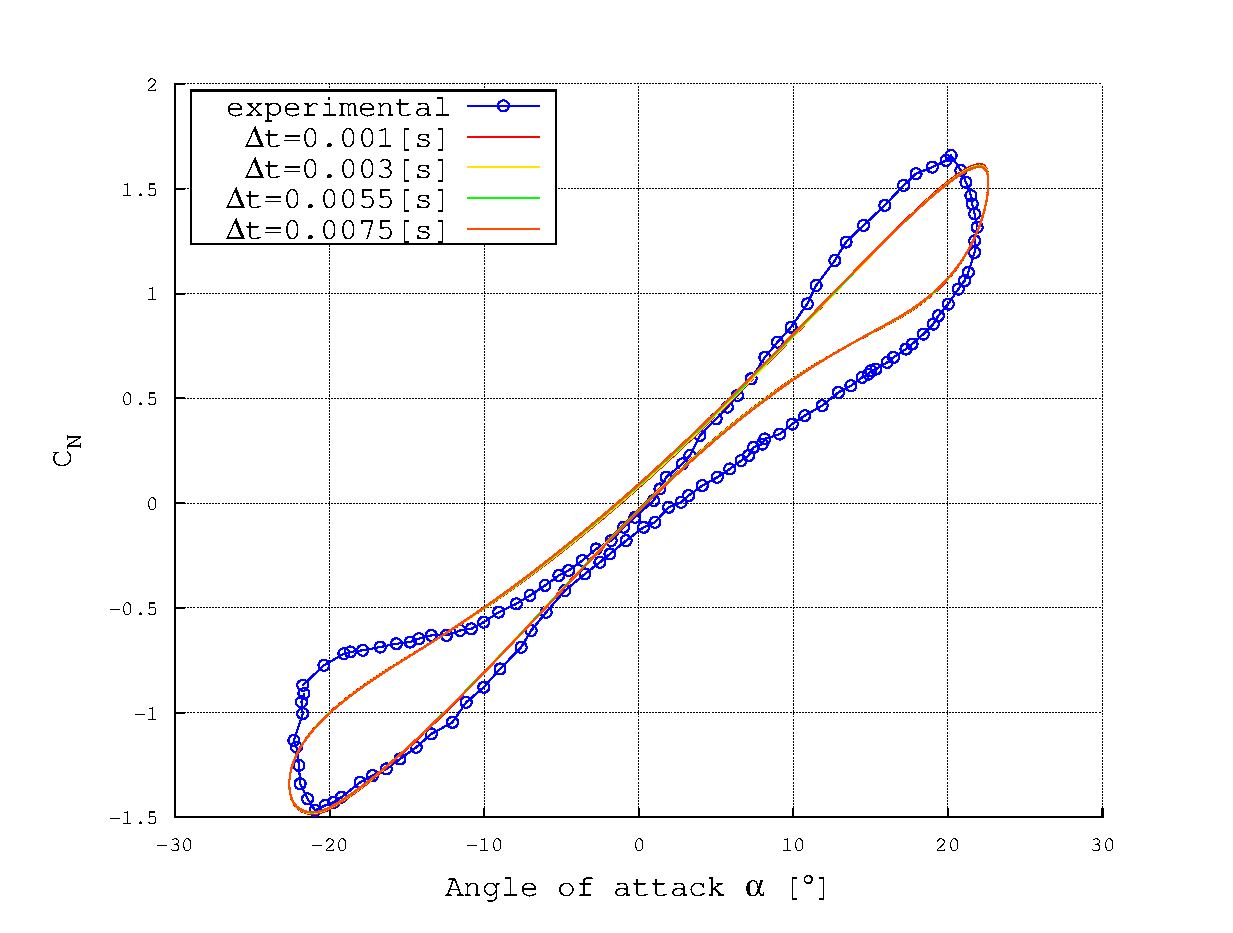
\includegraphics{CN226dtLEScoarse}}%
    \gplfronttext
  \end{picture}%
\endgroup
}
%\resizebox{\columnwidth}{!}{\input{plot}}
\end{minipage}\hspace{2pc}%
\begin{minipage}{18pc}
\resizebox{\columnwidth}{!}{% GNUPLOT: LaTeX picture with Postscript
\begingroup
  \makeatletter
  \providecommand\color[2][]{%
    \GenericError{(gnuplot) \space\space\space\@spaces}{%
      Package color not loaded in conjunction with
      terminal option `colourtext'%
    }{See the gnuplot documentation for explanation.%
    }{Either use 'blacktext' in gnuplot or load the package
      color.sty in LaTeX.}%
    \renewcommand\color[2][]{}%
  }%
  \providecommand\includegraphics[2][]{%
    \GenericError{(gnuplot) \space\space\space\@spaces}{%
      Package graphicx or graphics not loaded%
    }{See the gnuplot documentation for explanation.%
    }{The gnuplot epslatex terminal needs graphicx.sty or graphics.sty.}%
    \renewcommand\includegraphics[2][]{}%
  }%
  \providecommand\rotatebox[2]{#2}%
  \@ifundefined{ifGPcolor}{%
    \newif\ifGPcolor
    \GPcolorfalse
  }{}%
  \@ifundefined{ifGPblacktext}{%
    \newif\ifGPblacktext
    \GPblacktexttrue
  }{}%
  % define a \g@addto@macro without @ in the name:
  \let\gplgaddtomacro\g@addto@macro
  % define empty templates for all commands taking text:
  \gdef\gplbacktext{}%
  \gdef\gplfronttext{}%
  \makeatother
  \ifGPblacktext
    % no textcolor at all
    \def\colorrgb#1{}%
    \def\colorgray#1{}%
  \else
    % gray or color?
    \ifGPcolor
      \def\colorrgb#1{\color[rgb]{#1}}%
      \def\colorgray#1{\color[gray]{#1}}%
      \expandafter\def\csname LTw\endcsname{\color{white}}%
      \expandafter\def\csname LTb\endcsname{\color{black}}%
      \expandafter\def\csname LTa\endcsname{\color{black}}%
      \expandafter\def\csname LT0\endcsname{\color[rgb]{1,0,0}}%
      \expandafter\def\csname LT1\endcsname{\color[rgb]{0,1,0}}%
      \expandafter\def\csname LT2\endcsname{\color[rgb]{0,0,1}}%
      \expandafter\def\csname LT3\endcsname{\color[rgb]{1,0,1}}%
      \expandafter\def\csname LT4\endcsname{\color[rgb]{0,1,1}}%
      \expandafter\def\csname LT5\endcsname{\color[rgb]{1,1,0}}%
      \expandafter\def\csname LT6\endcsname{\color[rgb]{0,0,0}}%
      \expandafter\def\csname LT7\endcsname{\color[rgb]{1,0.3,0}}%
      \expandafter\def\csname LT8\endcsname{\color[rgb]{0.5,0.5,0.5}}%
    \else
      % gray
      \def\colorrgb#1{\color{black}}%
      \def\colorgray#1{\color[gray]{#1}}%
      \expandafter\def\csname LTw\endcsname{\color{white}}%
      \expandafter\def\csname LTb\endcsname{\color{black}}%
      \expandafter\def\csname LTa\endcsname{\color{black}}%
      \expandafter\def\csname LT0\endcsname{\color{black}}%
      \expandafter\def\csname LT1\endcsname{\color{black}}%
      \expandafter\def\csname LT2\endcsname{\color{black}}%
      \expandafter\def\csname LT3\endcsname{\color{black}}%
      \expandafter\def\csname LT4\endcsname{\color{black}}%
      \expandafter\def\csname LT5\endcsname{\color{black}}%
      \expandafter\def\csname LT6\endcsname{\color{black}}%
      \expandafter\def\csname LT7\endcsname{\color{black}}%
      \expandafter\def\csname LT8\endcsname{\color{black}}%
    \fi
  \fi
  \setlength{\unitlength}{0.0500bp}%
  \begin{picture}(7200.00,5040.00)%
    \gplgaddtomacro\gplbacktext{%
      \csname LTb\endcsname%
      \put(1078,704){\makebox(0,0)[r]{\strut{}-0.05}}%
      \csname LTb\endcsname%
      \put(1078,1111){\makebox(0,0)[r]{\strut{} 0}}%
      \csname LTb\endcsname%
      \put(1078,1518){\makebox(0,0)[r]{\strut{} 0.05}}%
      \csname LTb\endcsname%
      \put(1078,1925){\makebox(0,0)[r]{\strut{} 0.1}}%
      \csname LTb\endcsname%
      \put(1078,2332){\makebox(0,0)[r]{\strut{} 0.15}}%
      \csname LTb\endcsname%
      \put(1078,2740){\makebox(0,0)[r]{\strut{} 0.2}}%
      \csname LTb\endcsname%
      \put(1078,3147){\makebox(0,0)[r]{\strut{} 0.25}}%
      \csname LTb\endcsname%
      \put(1078,3554){\makebox(0,0)[r]{\strut{} 0.3}}%
      \csname LTb\endcsname%
      \put(1078,3961){\makebox(0,0)[r]{\strut{} 0.35}}%
      \csname LTb\endcsname%
      \put(1078,4368){\makebox(0,0)[r]{\strut{} 0.4}}%
      \csname LTb\endcsname%
      \put(1078,4775){\makebox(0,0)[r]{\strut{} 0.45}}%
      \csname LTb\endcsname%
      \put(1210,484){\makebox(0,0){\strut{}-25}}%
      \csname LTb\endcsname%
      \put(1769,484){\makebox(0,0){\strut{}-20}}%
      \csname LTb\endcsname%
      \put(2329,484){\makebox(0,0){\strut{}-15}}%
      \csname LTb\endcsname%
      \put(2888,484){\makebox(0,0){\strut{}-10}}%
      \csname LTb\endcsname%
      \put(3447,484){\makebox(0,0){\strut{}-5}}%
      \csname LTb\endcsname%
      \put(4007,484){\makebox(0,0){\strut{} 0}}%
      \csname LTb\endcsname%
      \put(4566,484){\makebox(0,0){\strut{} 5}}%
      \csname LTb\endcsname%
      \put(5125,484){\makebox(0,0){\strut{} 10}}%
      \csname LTb\endcsname%
      \put(5684,484){\makebox(0,0){\strut{} 15}}%
      \csname LTb\endcsname%
      \put(6244,484){\makebox(0,0){\strut{} 20}}%
      \csname LTb\endcsname%
      \put(6803,484){\makebox(0,0){\strut{} 25}}%
      \put(176,2739){\rotatebox{-270}{\makebox(0,0){\strut{}$C_T$}}}%
      \put(4006,154){\makebox(0,0){\strut{}Angle of attack {$\alpha$} [$\degree$]}}%
    }%
    \gplgaddtomacro\gplfronttext{%
      \csname LTb\endcsname%
      \put(4371,4602){\makebox(0,0)[r]{\strut{}experimental}}%
      \csname LTb\endcsname%
      \put(4371,4382){\makebox(0,0)[r]{\strut{}$\Delta$t=0.001[s]}}%
      \csname LTb\endcsname%
      \put(4371,4162){\makebox(0,0)[r]{\strut{}$\Delta$t=0.003[s]}}%
      \csname LTb\endcsname%
      \put(4371,3942){\makebox(0,0)[r]{\strut{}$\Delta$t=0.055[s]}}%
      \csname LTb\endcsname%
      \put(4371,3722){\makebox(0,0)[r]{\strut{}$\Delta$t=0.075[s]}}%
    }%
    \gplbacktext
    \put(0,0){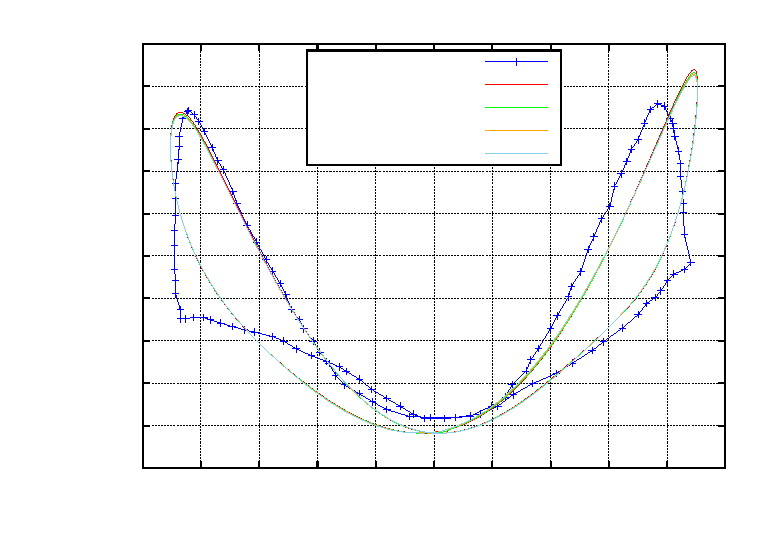
\includegraphics{CT226dtLEScoarse}}%
    \gplfronttext
  \end{picture}%
\endgroup
}
\end{minipage}
\caption{\label{figdtcoarse}Normal (left) and tangential (right) force coefficients varying time-step discretization for a pithing motion with a maximum amplitude of 22.6\degree\ }
\end{figure}

\subsection{TSR Variation}

For a TSR of 4.19 (Figure \ref{fig138}), peaks values for both $C_N$ and $C_T$
are similar to experiments. In this condition, the flow is attached and the
blades are not in the stall region. Therefore, model have good agreement with
experimental data using unsteady attached angle of attack calculation.

For a TSR of 3.34 (Figure \ref{fig174}), the maximum magnitude of the angle of
attack is at 17.4\degree\ which is in the stall region. Both $C_N$ and $C_T$
curves show the delay of the flow reattachment, which is characteristic of the
dynamic stall phenomenon. Peaks of simulated values have close agreement with
the measured data. The stall onset angle flow reattachment are well predicted.

For a TSR of 2.60 (Figure \ref{fig226}), the maximum amplitude of the angle of
attack is 22.6\degree, which is related to a deeper stall region compared to a
TSR of 3.34. This is shown because the ``loop'' of the curve is wider for the
lower TSR, and moreover, the reattachment of the flow is further delayed.
Simulated peak for $C_T$ is overestimated.

\begin{figure}[h]
\begin{minipage}{18pc}
\resizebox{\columnwidth}{!}{% GNUPLOT: LaTeX picture with Postscript
\begingroup
  \makeatletter
  \providecommand\color[2][]{%
    \GenericError{(gnuplot) \space\space\space\@spaces}{%
      Package color not loaded in conjunction with
      terminal option `colourtext'%
    }{See the gnuplot documentation for explanation.%
    }{Either use 'blacktext' in gnuplot or load the package
      color.sty in LaTeX.}%
    \renewcommand\color[2][]{}%
  }%
  \providecommand\includegraphics[2][]{%
    \GenericError{(gnuplot) \space\space\space\@spaces}{%
      Package graphicx or graphics not loaded%
    }{See the gnuplot documentation for explanation.%
    }{The gnuplot epslatex terminal needs graphicx.sty or graphics.sty.}%
    \renewcommand\includegraphics[2][]{}%
  }%
  \providecommand\rotatebox[2]{#2}%
  \@ifundefined{ifGPcolor}{%
    \newif\ifGPcolor
    \GPcolorfalse
  }{}%
  \@ifundefined{ifGPblacktext}{%
    \newif\ifGPblacktext
    \GPblacktexttrue
  }{}%
  % define a \g@addto@macro without @ in the name:
  \let\gplgaddtomacro\g@addto@macro
  % define empty templates for all commands taking text:
  \gdef\gplbacktext{}%
  \gdef\gplfronttext{}%
  \makeatother
  \ifGPblacktext
    % no textcolor at all
    \def\colorrgb#1{}%
    \def\colorgray#1{}%
  \else
    % gray or color?
    \ifGPcolor
      \def\colorrgb#1{\color[rgb]{#1}}%
      \def\colorgray#1{\color[gray]{#1}}%
      \expandafter\def\csname LTw\endcsname{\color{white}}%
      \expandafter\def\csname LTb\endcsname{\color{black}}%
      \expandafter\def\csname LTa\endcsname{\color{black}}%
      \expandafter\def\csname LT0\endcsname{\color[rgb]{1,0,0}}%
      \expandafter\def\csname LT1\endcsname{\color[rgb]{0,1,0}}%
      \expandafter\def\csname LT2\endcsname{\color[rgb]{0,0,1}}%
      \expandafter\def\csname LT3\endcsname{\color[rgb]{1,0,1}}%
      \expandafter\def\csname LT4\endcsname{\color[rgb]{0,1,1}}%
      \expandafter\def\csname LT5\endcsname{\color[rgb]{1,1,0}}%
      \expandafter\def\csname LT6\endcsname{\color[rgb]{0,0,0}}%
      \expandafter\def\csname LT7\endcsname{\color[rgb]{1,0.3,0}}%
      \expandafter\def\csname LT8\endcsname{\color[rgb]{0.5,0.5,0.5}}%
    \else
      % gray
      \def\colorrgb#1{\color{black}}%
      \def\colorgray#1{\color[gray]{#1}}%
      \expandafter\def\csname LTw\endcsname{\color{white}}%
      \expandafter\def\csname LTb\endcsname{\color{black}}%
      \expandafter\def\csname LTa\endcsname{\color{black}}%
      \expandafter\def\csname LT0\endcsname{\color{black}}%
      \expandafter\def\csname LT1\endcsname{\color{black}}%
      \expandafter\def\csname LT2\endcsname{\color{black}}%
      \expandafter\def\csname LT3\endcsname{\color{black}}%
      \expandafter\def\csname LT4\endcsname{\color{black}}%
      \expandafter\def\csname LT5\endcsname{\color{black}}%
      \expandafter\def\csname LT6\endcsname{\color{black}}%
      \expandafter\def\csname LT7\endcsname{\color{black}}%
      \expandafter\def\csname LT8\endcsname{\color{black}}%
    \fi
  \fi
  \setlength{\unitlength}{0.0500bp}%
  \begin{picture}(7200.00,5040.00)%
    \gplgaddtomacro\gplbacktext{%
      \csname LTb\endcsname%
      \put(946,704){\makebox(0,0)[r]{\strut{}-1.5}}%
      \csname LTb\endcsname%
      \put(946,1383){\makebox(0,0)[r]{\strut{}-1}}%
      \csname LTb\endcsname%
      \put(946,2061){\makebox(0,0)[r]{\strut{}-0.5}}%
      \csname LTb\endcsname%
      \put(946,2740){\makebox(0,0)[r]{\strut{} 0}}%
      \csname LTb\endcsname%
      \put(946,3418){\makebox(0,0)[r]{\strut{} 0.5}}%
      \csname LTb\endcsname%
      \put(946,4097){\makebox(0,0)[r]{\strut{} 1}}%
      \csname LTb\endcsname%
      \put(946,4775){\makebox(0,0)[r]{\strut{} 1.5}}%
      \csname LTb\endcsname%
      \put(1078,484){\makebox(0,0){\strut{}-15}}%
      \csname LTb\endcsname%
      \put(2032,484){\makebox(0,0){\strut{}-10}}%
      \csname LTb\endcsname%
      \put(2986,484){\makebox(0,0){\strut{}-5}}%
      \csname LTb\endcsname%
      \put(3941,484){\makebox(0,0){\strut{} 0}}%
      \csname LTb\endcsname%
      \put(4895,484){\makebox(0,0){\strut{} 5}}%
      \csname LTb\endcsname%
      \put(5849,484){\makebox(0,0){\strut{} 10}}%
      \csname LTb\endcsname%
      \put(6803,484){\makebox(0,0){\strut{} 15}}%
      \put(176,2739){\rotatebox{-270}{\makebox(0,0){\strut{}$C_N$}}}%
      \put(3940,154){\makebox(0,0){\strut{}Angle of attack {$\alpha$} [$\degree$]}}%
    }%
    \gplgaddtomacro\gplfronttext{%
      \csname LTb\endcsname%
      \put(2794,4602){\makebox(0,0)[r]{\strut{}experimental}}%
      \csname LTb\endcsname%
      \put(2794,4382){\makebox(0,0)[r]{\strut{}simulated}}%
    }%
    \gplbacktext
    \put(0,0){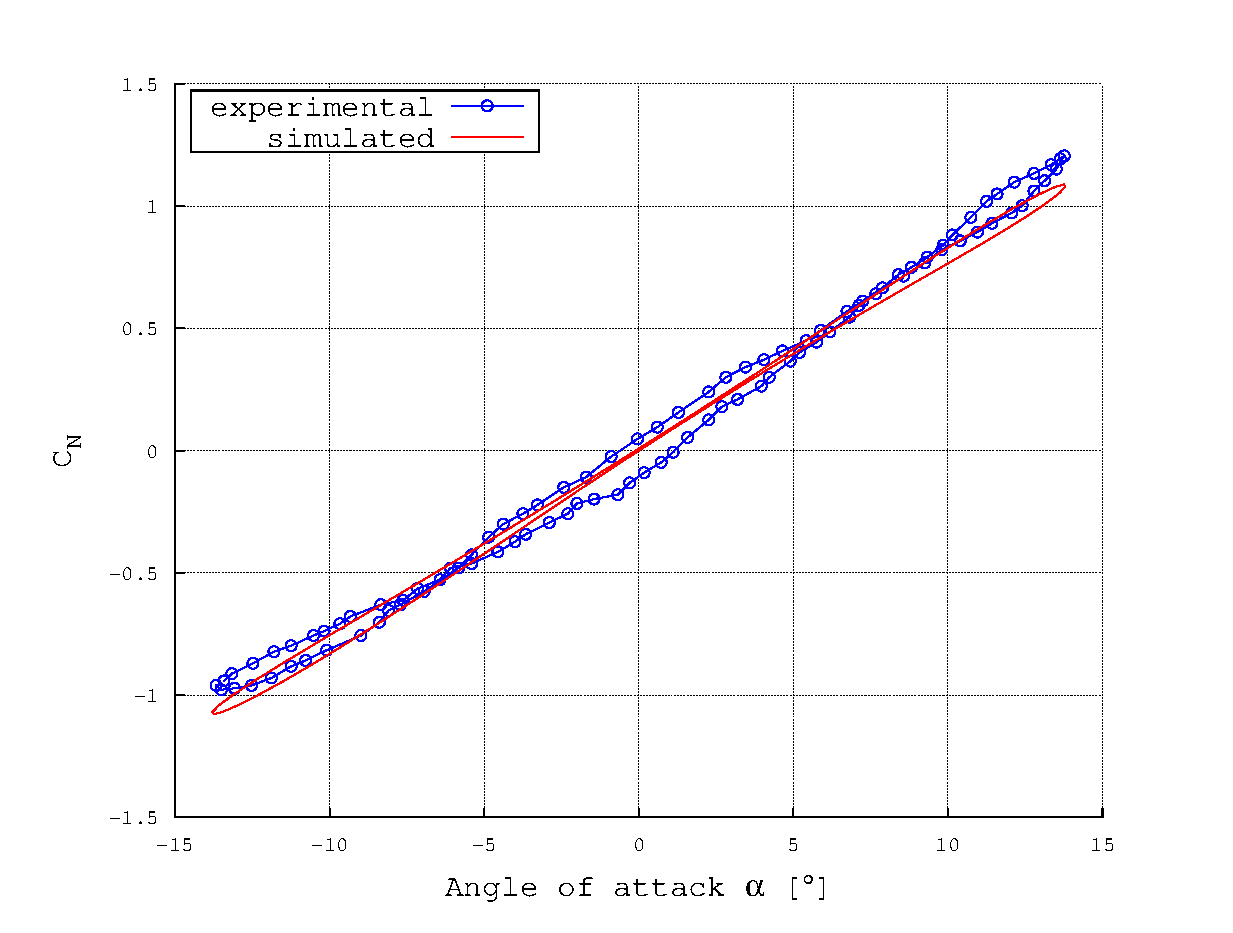
\includegraphics{CN138}}%
    \gplfronttext
  \end{picture}%
\endgroup
}
%\resizebox{\columnwidth}{!}{\input{plot}}
\end{minipage}\hspace{2pc}%
\begin{minipage}{18pc}
\resizebox{\columnwidth}{!}{% GNUPLOT: LaTeX picture with Postscript
\begingroup
  \makeatletter
  \providecommand\color[2][]{%
    \GenericError{(gnuplot) \space\space\space\@spaces}{%
      Package color not loaded in conjunction with
      terminal option `colourtext'%
    }{See the gnuplot documentation for explanation.%
    }{Either use 'blacktext' in gnuplot or load the package
      color.sty in LaTeX.}%
    \renewcommand\color[2][]{}%
  }%
  \providecommand\includegraphics[2][]{%
    \GenericError{(gnuplot) \space\space\space\@spaces}{%
      Package graphicx or graphics not loaded%
    }{See the gnuplot documentation for explanation.%
    }{The gnuplot epslatex terminal needs graphicx.sty or graphics.sty.}%
    \renewcommand\includegraphics[2][]{}%
  }%
  \providecommand\rotatebox[2]{#2}%
  \@ifundefined{ifGPcolor}{%
    \newif\ifGPcolor
    \GPcolorfalse
  }{}%
  \@ifundefined{ifGPblacktext}{%
    \newif\ifGPblacktext
    \GPblacktexttrue
  }{}%
  % define a \g@addto@macro without @ in the name:
  \let\gplgaddtomacro\g@addto@macro
  % define empty templates for all commands taking text:
  \gdef\gplbacktext{}%
  \gdef\gplfronttext{}%
  \makeatother
  \ifGPblacktext
    % no textcolor at all
    \def\colorrgb#1{}%
    \def\colorgray#1{}%
  \else
    % gray or color?
    \ifGPcolor
      \def\colorrgb#1{\color[rgb]{#1}}%
      \def\colorgray#1{\color[gray]{#1}}%
      \expandafter\def\csname LTw\endcsname{\color{white}}%
      \expandafter\def\csname LTb\endcsname{\color{black}}%
      \expandafter\def\csname LTa\endcsname{\color{black}}%
      \expandafter\def\csname LT0\endcsname{\color[rgb]{1,0,0}}%
      \expandafter\def\csname LT1\endcsname{\color[rgb]{0,1,0}}%
      \expandafter\def\csname LT2\endcsname{\color[rgb]{0,0,1}}%
      \expandafter\def\csname LT3\endcsname{\color[rgb]{1,0,1}}%
      \expandafter\def\csname LT4\endcsname{\color[rgb]{0,1,1}}%
      \expandafter\def\csname LT5\endcsname{\color[rgb]{1,1,0}}%
      \expandafter\def\csname LT6\endcsname{\color[rgb]{0,0,0}}%
      \expandafter\def\csname LT7\endcsname{\color[rgb]{1,0.3,0}}%
      \expandafter\def\csname LT8\endcsname{\color[rgb]{0.5,0.5,0.5}}%
    \else
      % gray
      \def\colorrgb#1{\color{black}}%
      \def\colorgray#1{\color[gray]{#1}}%
      \expandafter\def\csname LTw\endcsname{\color{white}}%
      \expandafter\def\csname LTb\endcsname{\color{black}}%
      \expandafter\def\csname LTa\endcsname{\color{black}}%
      \expandafter\def\csname LT0\endcsname{\color{black}}%
      \expandafter\def\csname LT1\endcsname{\color{black}}%
      \expandafter\def\csname LT2\endcsname{\color{black}}%
      \expandafter\def\csname LT3\endcsname{\color{black}}%
      \expandafter\def\csname LT4\endcsname{\color{black}}%
      \expandafter\def\csname LT5\endcsname{\color{black}}%
      \expandafter\def\csname LT6\endcsname{\color{black}}%
      \expandafter\def\csname LT7\endcsname{\color{black}}%
      \expandafter\def\csname LT8\endcsname{\color{black}}%
    \fi
  \fi
  \setlength{\unitlength}{0.0500bp}%
  \begin{picture}(7200.00,5040.00)%
    \gplgaddtomacro\gplbacktext{%
      \csname LTb\endcsname%
      \put(1078,704){\makebox(0,0)[r]{\strut{}-0.05}}%
      \csname LTb\endcsname%
      \put(1078,1383){\makebox(0,0)[r]{\strut{} 0}}%
      \csname LTb\endcsname%
      \put(1078,2061){\makebox(0,0)[r]{\strut{} 0.05}}%
      \csname LTb\endcsname%
      \put(1078,2740){\makebox(0,0)[r]{\strut{} 0.1}}%
      \csname LTb\endcsname%
      \put(1078,3418){\makebox(0,0)[r]{\strut{} 0.15}}%
      \csname LTb\endcsname%
      \put(1078,4097){\makebox(0,0)[r]{\strut{} 0.2}}%
      \csname LTb\endcsname%
      \put(1078,4775){\makebox(0,0)[r]{\strut{} 0.25}}%
      \csname LTb\endcsname%
      \put(1210,484){\makebox(0,0){\strut{}-15}}%
      \csname LTb\endcsname%
      \put(2142,484){\makebox(0,0){\strut{}-10}}%
      \csname LTb\endcsname%
      \put(3074,484){\makebox(0,0){\strut{}-5}}%
      \csname LTb\endcsname%
      \put(4007,484){\makebox(0,0){\strut{} 0}}%
      \csname LTb\endcsname%
      \put(4939,484){\makebox(0,0){\strut{} 5}}%
      \csname LTb\endcsname%
      \put(5871,484){\makebox(0,0){\strut{} 10}}%
      \csname LTb\endcsname%
      \put(6803,484){\makebox(0,0){\strut{} 15}}%
      \put(176,2739){\rotatebox{-270}{\makebox(0,0){\strut{}$C_T$}}}%
      \put(4006,154){\makebox(0,0){\strut{}Angle of attack {$\alpha$} [$\degree$]}}%
    }%
    \gplgaddtomacro\gplfronttext{%
      \csname LTb\endcsname%
      \put(4371,4602){\makebox(0,0)[r]{\strut{}experimental}}%
      \csname LTb\endcsname%
      \put(4371,4382){\makebox(0,0)[r]{\strut{}simulated}}%
    }%
    \gplbacktext
    \put(0,0){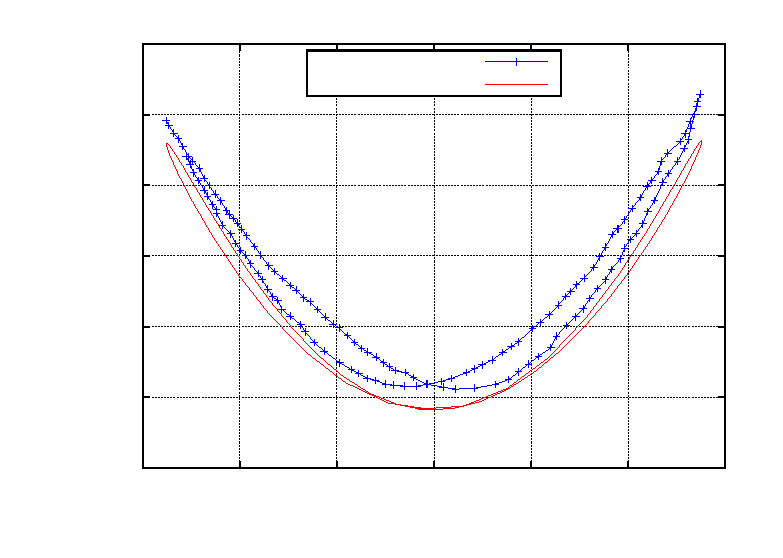
\includegraphics{CT138}}%
    \gplfronttext
  \end{picture}%
\endgroup
}
\end{minipage}
\caption{\label{fig138}Normal (left) and tangential (right) force coefficients during pitching motions of NACA0021 airfoil with a maximum amplitude of 13.8\degree\ (analog to $\lambda = 4.19$).}
\end{figure}


\begin{figure}[h]
\begin{minipage}{18pc}
\resizebox{\columnwidth}{!}{% GNUPLOT: LaTeX picture with Postscript
\begingroup
  \makeatletter
  \providecommand\color[2][]{%
    \GenericError{(gnuplot) \space\space\space\@spaces}{%
      Package color not loaded in conjunction with
      terminal option `colourtext'%
    }{See the gnuplot documentation for explanation.%
    }{Either use 'blacktext' in gnuplot or load the package
      color.sty in LaTeX.}%
    \renewcommand\color[2][]{}%
  }%
  \providecommand\includegraphics[2][]{%
    \GenericError{(gnuplot) \space\space\space\@spaces}{%
      Package graphicx or graphics not loaded%
    }{See the gnuplot documentation for explanation.%
    }{The gnuplot epslatex terminal needs graphicx.sty or graphics.sty.}%
    \renewcommand\includegraphics[2][]{}%
  }%
  \providecommand\rotatebox[2]{#2}%
  \@ifundefined{ifGPcolor}{%
    \newif\ifGPcolor
    \GPcolorfalse
  }{}%
  \@ifundefined{ifGPblacktext}{%
    \newif\ifGPblacktext
    \GPblacktexttrue
  }{}%
  % define a \g@addto@macro without @ in the name:
  \let\gplgaddtomacro\g@addto@macro
  % define empty templates for all commands taking text:
  \gdef\gplbacktext{}%
  \gdef\gplfronttext{}%
  \makeatother
  \ifGPblacktext
    % no textcolor at all
    \def\colorrgb#1{}%
    \def\colorgray#1{}%
  \else
    % gray or color?
    \ifGPcolor
      \def\colorrgb#1{\color[rgb]{#1}}%
      \def\colorgray#1{\color[gray]{#1}}%
      \expandafter\def\csname LTw\endcsname{\color{white}}%
      \expandafter\def\csname LTb\endcsname{\color{black}}%
      \expandafter\def\csname LTa\endcsname{\color{black}}%
      \expandafter\def\csname LT0\endcsname{\color[rgb]{1,0,0}}%
      \expandafter\def\csname LT1\endcsname{\color[rgb]{0,1,0}}%
      \expandafter\def\csname LT2\endcsname{\color[rgb]{0,0,1}}%
      \expandafter\def\csname LT3\endcsname{\color[rgb]{1,0,1}}%
      \expandafter\def\csname LT4\endcsname{\color[rgb]{0,1,1}}%
      \expandafter\def\csname LT5\endcsname{\color[rgb]{1,1,0}}%
      \expandafter\def\csname LT6\endcsname{\color[rgb]{0,0,0}}%
      \expandafter\def\csname LT7\endcsname{\color[rgb]{1,0.3,0}}%
      \expandafter\def\csname LT8\endcsname{\color[rgb]{0.5,0.5,0.5}}%
    \else
      % gray
      \def\colorrgb#1{\color{black}}%
      \def\colorgray#1{\color[gray]{#1}}%
      \expandafter\def\csname LTw\endcsname{\color{white}}%
      \expandafter\def\csname LTb\endcsname{\color{black}}%
      \expandafter\def\csname LTa\endcsname{\color{black}}%
      \expandafter\def\csname LT0\endcsname{\color{black}}%
      \expandafter\def\csname LT1\endcsname{\color{black}}%
      \expandafter\def\csname LT2\endcsname{\color{black}}%
      \expandafter\def\csname LT3\endcsname{\color{black}}%
      \expandafter\def\csname LT4\endcsname{\color{black}}%
      \expandafter\def\csname LT5\endcsname{\color{black}}%
      \expandafter\def\csname LT6\endcsname{\color{black}}%
      \expandafter\def\csname LT7\endcsname{\color{black}}%
      \expandafter\def\csname LT8\endcsname{\color{black}}%
    \fi
  \fi
  \setlength{\unitlength}{0.0500bp}%
  \begin{picture}(7200.00,5040.00)%
    \gplgaddtomacro\gplbacktext{%
      \csname LTb\endcsname%
      \put(946,704){\makebox(0,0)[r]{\strut{}-1.5}}%
      \csname LTb\endcsname%
      \put(946,1383){\makebox(0,0)[r]{\strut{}-1}}%
      \csname LTb\endcsname%
      \put(946,2061){\makebox(0,0)[r]{\strut{}-0.5}}%
      \csname LTb\endcsname%
      \put(946,2740){\makebox(0,0)[r]{\strut{} 0}}%
      \csname LTb\endcsname%
      \put(946,3418){\makebox(0,0)[r]{\strut{} 0.5}}%
      \csname LTb\endcsname%
      \put(946,4097){\makebox(0,0)[r]{\strut{} 1}}%
      \csname LTb\endcsname%
      \put(946,4775){\makebox(0,0)[r]{\strut{} 1.5}}%
      \csname LTb\endcsname%
      \put(1078,484){\makebox(0,0){\strut{}-20}}%
      \csname LTb\endcsname%
      \put(1794,484){\makebox(0,0){\strut{}-15}}%
      \csname LTb\endcsname%
      \put(2509,484){\makebox(0,0){\strut{}-10}}%
      \csname LTb\endcsname%
      \put(3225,484){\makebox(0,0){\strut{}-5}}%
      \csname LTb\endcsname%
      \put(3941,484){\makebox(0,0){\strut{} 0}}%
      \csname LTb\endcsname%
      \put(4656,484){\makebox(0,0){\strut{} 5}}%
      \csname LTb\endcsname%
      \put(5372,484){\makebox(0,0){\strut{} 10}}%
      \csname LTb\endcsname%
      \put(6087,484){\makebox(0,0){\strut{} 15}}%
      \csname LTb\endcsname%
      \put(6803,484){\makebox(0,0){\strut{} 20}}%
      \put(176,2739){\rotatebox{-270}{\makebox(0,0){\strut{}$C_N$}}}%
      \put(3940,154){\makebox(0,0){\strut{}Angle of attack {$\alpha$} [$\degree$]}}%
    }%
    \gplgaddtomacro\gplfronttext{%
      \csname LTb\endcsname%
      \put(2794,4602){\makebox(0,0)[r]{\strut{}experimental}}%
      \csname LTb\endcsname%
      \put(2794,4382){\makebox(0,0)[r]{\strut{}simulated}}%
    }%
    \gplbacktext
    \put(0,0){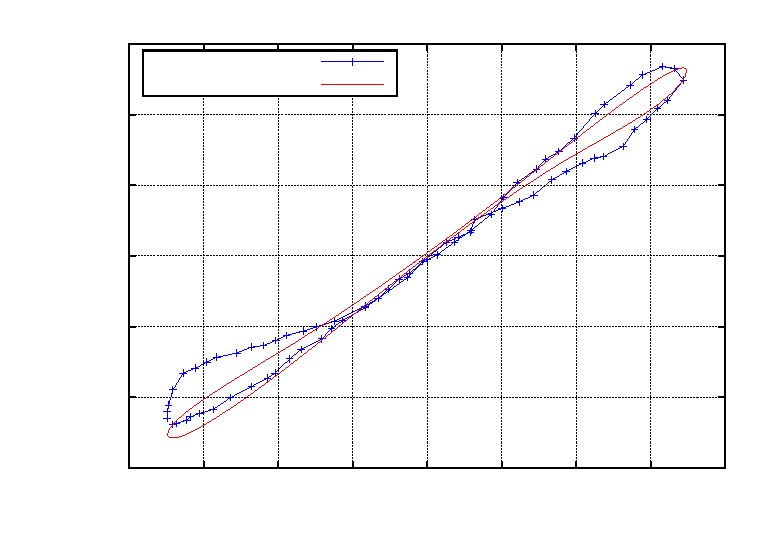
\includegraphics{CN174}}%
    \gplfronttext
  \end{picture}%
\endgroup
}
%\resizebox{\columnwidth}{!}{\input{plot}}
\end{minipage}\hspace{2pc}%
\begin{minipage}{18pc}
\resizebox{\columnwidth}{!}{% GNUPLOT: LaTeX picture with Postscript
\begingroup
  \makeatletter
  \providecommand\color[2][]{%
    \GenericError{(gnuplot) \space\space\space\@spaces}{%
      Package color not loaded in conjunction with
      terminal option `colourtext'%
    }{See the gnuplot documentation for explanation.%
    }{Either use 'blacktext' in gnuplot or load the package
      color.sty in LaTeX.}%
    \renewcommand\color[2][]{}%
  }%
  \providecommand\includegraphics[2][]{%
    \GenericError{(gnuplot) \space\space\space\@spaces}{%
      Package graphicx or graphics not loaded%
    }{See the gnuplot documentation for explanation.%
    }{The gnuplot epslatex terminal needs graphicx.sty or graphics.sty.}%
    \renewcommand\includegraphics[2][]{}%
  }%
  \providecommand\rotatebox[2]{#2}%
  \@ifundefined{ifGPcolor}{%
    \newif\ifGPcolor
    \GPcolorfalse
  }{}%
  \@ifundefined{ifGPblacktext}{%
    \newif\ifGPblacktext
    \GPblacktexttrue
  }{}%
  % define a \g@addto@macro without @ in the name:
  \let\gplgaddtomacro\g@addto@macro
  % define empty templates for all commands taking text:
  \gdef\gplbacktext{}%
  \gdef\gplfronttext{}%
  \makeatother
  \ifGPblacktext
    % no textcolor at all
    \def\colorrgb#1{}%
    \def\colorgray#1{}%
  \else
    % gray or color?
    \ifGPcolor
      \def\colorrgb#1{\color[rgb]{#1}}%
      \def\colorgray#1{\color[gray]{#1}}%
      \expandafter\def\csname LTw\endcsname{\color{white}}%
      \expandafter\def\csname LTb\endcsname{\color{black}}%
      \expandafter\def\csname LTa\endcsname{\color{black}}%
      \expandafter\def\csname LT0\endcsname{\color[rgb]{1,0,0}}%
      \expandafter\def\csname LT1\endcsname{\color[rgb]{0,1,0}}%
      \expandafter\def\csname LT2\endcsname{\color[rgb]{0,0,1}}%
      \expandafter\def\csname LT3\endcsname{\color[rgb]{1,0,1}}%
      \expandafter\def\csname LT4\endcsname{\color[rgb]{0,1,1}}%
      \expandafter\def\csname LT5\endcsname{\color[rgb]{1,1,0}}%
      \expandafter\def\csname LT6\endcsname{\color[rgb]{0,0,0}}%
      \expandafter\def\csname LT7\endcsname{\color[rgb]{1,0.3,0}}%
      \expandafter\def\csname LT8\endcsname{\color[rgb]{0.5,0.5,0.5}}%
    \else
      % gray
      \def\colorrgb#1{\color{black}}%
      \def\colorgray#1{\color[gray]{#1}}%
      \expandafter\def\csname LTw\endcsname{\color{white}}%
      \expandafter\def\csname LTb\endcsname{\color{black}}%
      \expandafter\def\csname LTa\endcsname{\color{black}}%
      \expandafter\def\csname LT0\endcsname{\color{black}}%
      \expandafter\def\csname LT1\endcsname{\color{black}}%
      \expandafter\def\csname LT2\endcsname{\color{black}}%
      \expandafter\def\csname LT3\endcsname{\color{black}}%
      \expandafter\def\csname LT4\endcsname{\color{black}}%
      \expandafter\def\csname LT5\endcsname{\color{black}}%
      \expandafter\def\csname LT6\endcsname{\color{black}}%
      \expandafter\def\csname LT7\endcsname{\color{black}}%
      \expandafter\def\csname LT8\endcsname{\color{black}}%
    \fi
  \fi
  \setlength{\unitlength}{0.0500bp}%
  \begin{picture}(7200.00,5040.00)%
    \gplgaddtomacro\gplbacktext{%
      \csname LTb\endcsname%
      \put(1078,704){\makebox(0,0)[r]{\strut{}-0.05}}%
      \csname LTb\endcsname%
      \put(1078,1286){\makebox(0,0)[r]{\strut{} 0}}%
      \csname LTb\endcsname%
      \put(1078,1867){\makebox(0,0)[r]{\strut{} 0.05}}%
      \csname LTb\endcsname%
      \put(1078,2449){\makebox(0,0)[r]{\strut{} 0.1}}%
      \csname LTb\endcsname%
      \put(1078,3030){\makebox(0,0)[r]{\strut{} 0.15}}%
      \csname LTb\endcsname%
      \put(1078,3612){\makebox(0,0)[r]{\strut{} 0.2}}%
      \csname LTb\endcsname%
      \put(1078,4193){\makebox(0,0)[r]{\strut{} 0.25}}%
      \csname LTb\endcsname%
      \put(1078,4775){\makebox(0,0)[r]{\strut{} 0.3}}%
      \csname LTb\endcsname%
      \put(1210,484){\makebox(0,0){\strut{}-20}}%
      \csname LTb\endcsname%
      \put(1909,484){\makebox(0,0){\strut{}-15}}%
      \csname LTb\endcsname%
      \put(2608,484){\makebox(0,0){\strut{}-10}}%
      \csname LTb\endcsname%
      \put(3307,484){\makebox(0,0){\strut{}-5}}%
      \csname LTb\endcsname%
      \put(4007,484){\makebox(0,0){\strut{} 0}}%
      \csname LTb\endcsname%
      \put(4706,484){\makebox(0,0){\strut{} 5}}%
      \csname LTb\endcsname%
      \put(5405,484){\makebox(0,0){\strut{} 10}}%
      \csname LTb\endcsname%
      \put(6104,484){\makebox(0,0){\strut{} 15}}%
      \csname LTb\endcsname%
      \put(6803,484){\makebox(0,0){\strut{} 20}}%
      \put(176,2739){\rotatebox{-270}{\makebox(0,0){\strut{}$C_T$}}}%
      \put(4006,154){\makebox(0,0){\strut{}Angle of attack {$\alpha$} [$\degree$]}}%
    }%
    \gplgaddtomacro\gplfronttext{%
      \csname LTb\endcsname%
      \put(4371,4602){\makebox(0,0)[r]{\strut{}experimental}}%
      \csname LTb\endcsname%
      \put(4371,4382){\makebox(0,0)[r]{\strut{}simulated}}%
    }%
    \gplbacktext
    \put(0,0){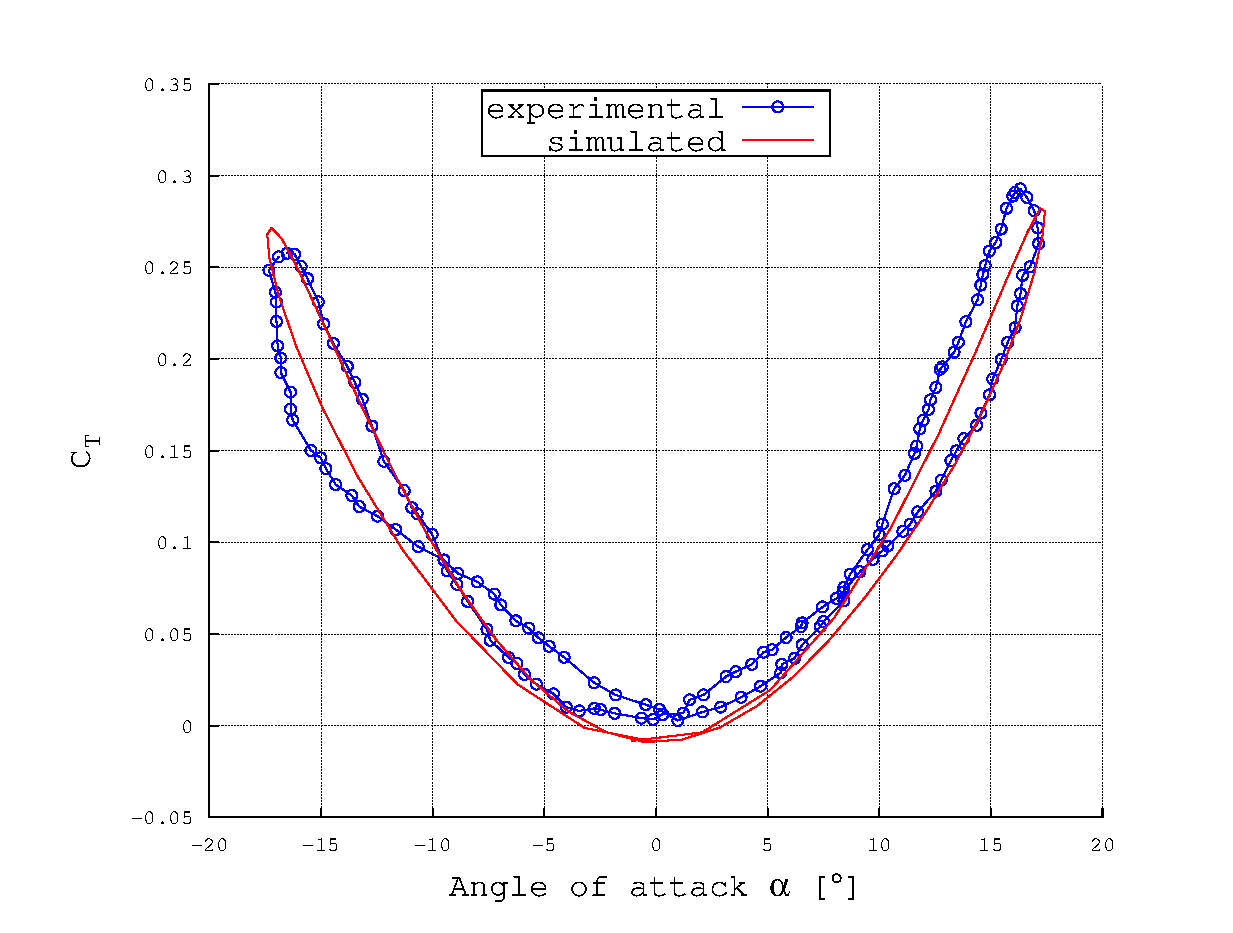
\includegraphics{CT174}}%
    \gplfronttext
  \end{picture}%
\endgroup
}
\end{minipage}
\caption{\label{fig174}Normal (left) and tangential (right) force coefficients during pitching motions of NACA0021 airfoil with a maximum amplitude of 17.4\degree\ (analog to $\lambda = 3.34$).}
\end{figure}

\begin{figure}[h]
\begin{minipage}{18pc}
\resizebox{\columnwidth}{!}{% GNUPLOT: LaTeX picture with Postscript
\begingroup
  \makeatletter
  \providecommand\color[2][]{%
    \GenericError{(gnuplot) \space\space\space\@spaces}{%
      Package color not loaded in conjunction with
      terminal option `colourtext'%
    }{See the gnuplot documentation for explanation.%
    }{Either use 'blacktext' in gnuplot or load the package
      color.sty in LaTeX.}%
    \renewcommand\color[2][]{}%
  }%
  \providecommand\includegraphics[2][]{%
    \GenericError{(gnuplot) \space\space\space\@spaces}{%
      Package graphicx or graphics not loaded%
    }{See the gnuplot documentation for explanation.%
    }{The gnuplot epslatex terminal needs graphicx.sty or graphics.sty.}%
    \renewcommand\includegraphics[2][]{}%
  }%
  \providecommand\rotatebox[2]{#2}%
  \@ifundefined{ifGPcolor}{%
    \newif\ifGPcolor
    \GPcolorfalse
  }{}%
  \@ifundefined{ifGPblacktext}{%
    \newif\ifGPblacktext
    \GPblacktexttrue
  }{}%
  % define a \g@addto@macro without @ in the name:
  \let\gplgaddtomacro\g@addto@macro
  % define empty templates for all commands taking text:
  \gdef\gplbacktext{}%
  \gdef\gplfronttext{}%
  \makeatother
  \ifGPblacktext
    % no textcolor at all
    \def\colorrgb#1{}%
    \def\colorgray#1{}%
  \else
    % gray or color?
    \ifGPcolor
      \def\colorrgb#1{\color[rgb]{#1}}%
      \def\colorgray#1{\color[gray]{#1}}%
      \expandafter\def\csname LTw\endcsname{\color{white}}%
      \expandafter\def\csname LTb\endcsname{\color{black}}%
      \expandafter\def\csname LTa\endcsname{\color{black}}%
      \expandafter\def\csname LT0\endcsname{\color[rgb]{1,0,0}}%
      \expandafter\def\csname LT1\endcsname{\color[rgb]{0,1,0}}%
      \expandafter\def\csname LT2\endcsname{\color[rgb]{0,0,1}}%
      \expandafter\def\csname LT3\endcsname{\color[rgb]{1,0,1}}%
      \expandafter\def\csname LT4\endcsname{\color[rgb]{0,1,1}}%
      \expandafter\def\csname LT5\endcsname{\color[rgb]{1,1,0}}%
      \expandafter\def\csname LT6\endcsname{\color[rgb]{0,0,0}}%
      \expandafter\def\csname LT7\endcsname{\color[rgb]{1,0.3,0}}%
      \expandafter\def\csname LT8\endcsname{\color[rgb]{0.5,0.5,0.5}}%
    \else
      % gray
      \def\colorrgb#1{\color{black}}%
      \def\colorgray#1{\color[gray]{#1}}%
      \expandafter\def\csname LTw\endcsname{\color{white}}%
      \expandafter\def\csname LTb\endcsname{\color{black}}%
      \expandafter\def\csname LTa\endcsname{\color{black}}%
      \expandafter\def\csname LT0\endcsname{\color{black}}%
      \expandafter\def\csname LT1\endcsname{\color{black}}%
      \expandafter\def\csname LT2\endcsname{\color{black}}%
      \expandafter\def\csname LT3\endcsname{\color{black}}%
      \expandafter\def\csname LT4\endcsname{\color{black}}%
      \expandafter\def\csname LT5\endcsname{\color{black}}%
      \expandafter\def\csname LT6\endcsname{\color{black}}%
      \expandafter\def\csname LT7\endcsname{\color{black}}%
      \expandafter\def\csname LT8\endcsname{\color{black}}%
    \fi
  \fi
  \setlength{\unitlength}{0.0500bp}%
  \begin{picture}(7200.00,5040.00)%
    \gplgaddtomacro\gplbacktext{%
      \csname LTb\endcsname%
      \put(946,704){\makebox(0,0)[r]{\strut{}-2}}%
      \csname LTb\endcsname%
      \put(946,1213){\makebox(0,0)[r]{\strut{}-1.5}}%
      \csname LTb\endcsname%
      \put(946,1722){\makebox(0,0)[r]{\strut{}-1}}%
      \csname LTb\endcsname%
      \put(946,2231){\makebox(0,0)[r]{\strut{}-0.5}}%
      \csname LTb\endcsname%
      \put(946,2740){\makebox(0,0)[r]{\strut{} 0}}%
      \csname LTb\endcsname%
      \put(946,3248){\makebox(0,0)[r]{\strut{} 0.5}}%
      \csname LTb\endcsname%
      \put(946,3757){\makebox(0,0)[r]{\strut{} 1}}%
      \csname LTb\endcsname%
      \put(946,4266){\makebox(0,0)[r]{\strut{} 1.5}}%
      \csname LTb\endcsname%
      \put(946,4775){\makebox(0,0)[r]{\strut{} 2}}%
      \csname LTb\endcsname%
      \put(1078,484){\makebox(0,0){\strut{}-25}}%
      \csname LTb\endcsname%
      \put(1651,484){\makebox(0,0){\strut{}-20}}%
      \csname LTb\endcsname%
      \put(2223,484){\makebox(0,0){\strut{}-15}}%
      \csname LTb\endcsname%
      \put(2796,484){\makebox(0,0){\strut{}-10}}%
      \csname LTb\endcsname%
      \put(3368,484){\makebox(0,0){\strut{}-5}}%
      \csname LTb\endcsname%
      \put(3941,484){\makebox(0,0){\strut{} 0}}%
      \csname LTb\endcsname%
      \put(4513,484){\makebox(0,0){\strut{} 5}}%
      \csname LTb\endcsname%
      \put(5086,484){\makebox(0,0){\strut{} 10}}%
      \csname LTb\endcsname%
      \put(5658,484){\makebox(0,0){\strut{} 15}}%
      \csname LTb\endcsname%
      \put(6231,484){\makebox(0,0){\strut{} 20}}%
      \csname LTb\endcsname%
      \put(6803,484){\makebox(0,0){\strut{} 25}}%
      \put(176,2739){\rotatebox{-270}{\makebox(0,0){\strut{}$C_N$}}}%
      \put(3940,154){\makebox(0,0){\strut{}Angle of attack {$\alpha$} [$\degree$]}}%
    }%
    \gplgaddtomacro\gplfronttext{%
      \csname LTb\endcsname%
      \put(2794,4602){\makebox(0,0)[r]{\strut{}experimental}}%
      \csname LTb\endcsname%
      \put(2794,4382){\makebox(0,0)[r]{\strut{}simulated}}%
    }%
    \gplbacktext
    \put(0,0){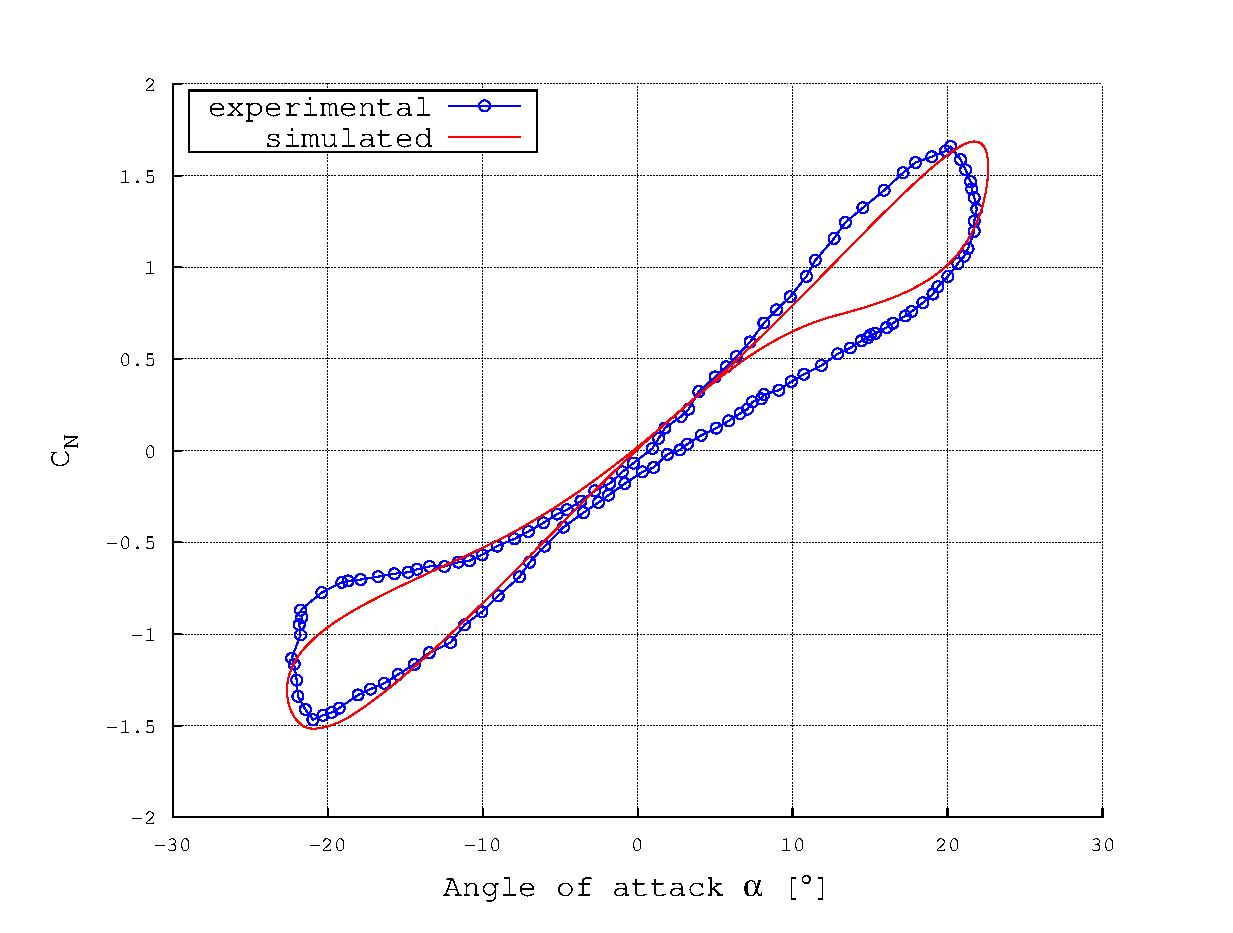
\includegraphics{CN226}}%
    \gplfronttext
  \end{picture}%
\endgroup
}
%\resizebox{\columnwidth}{!}{\input{plot}}
\end{minipage}\hspace{2pc}%
\begin{minipage}{18pc}
\resizebox{\columnwidth}{!}{% GNUPLOT: LaTeX picture with Postscript
\begingroup
  \makeatletter
  \providecommand\color[2][]{%
    \GenericError{(gnuplot) \space\space\space\@spaces}{%
      Package color not loaded in conjunction with
      terminal option `colourtext'%
    }{See the gnuplot documentation for explanation.%
    }{Either use 'blacktext' in gnuplot or load the package
      color.sty in LaTeX.}%
    \renewcommand\color[2][]{}%
  }%
  \providecommand\includegraphics[2][]{%
    \GenericError{(gnuplot) \space\space\space\@spaces}{%
      Package graphicx or graphics not loaded%
    }{See the gnuplot documentation for explanation.%
    }{The gnuplot epslatex terminal needs graphicx.sty or graphics.sty.}%
    \renewcommand\includegraphics[2][]{}%
  }%
  \providecommand\rotatebox[2]{#2}%
  \@ifundefined{ifGPcolor}{%
    \newif\ifGPcolor
    \GPcolorfalse
  }{}%
  \@ifundefined{ifGPblacktext}{%
    \newif\ifGPblacktext
    \GPblacktexttrue
  }{}%
  % define a \g@addto@macro without @ in the name:
  \let\gplgaddtomacro\g@addto@macro
  % define empty templates for all commands taking text:
  \gdef\gplbacktext{}%
  \gdef\gplfronttext{}%
  \makeatother
  \ifGPblacktext
    % no textcolor at all
    \def\colorrgb#1{}%
    \def\colorgray#1{}%
  \else
    % gray or color?
    \ifGPcolor
      \def\colorrgb#1{\color[rgb]{#1}}%
      \def\colorgray#1{\color[gray]{#1}}%
      \expandafter\def\csname LTw\endcsname{\color{white}}%
      \expandafter\def\csname LTb\endcsname{\color{black}}%
      \expandafter\def\csname LTa\endcsname{\color{black}}%
      \expandafter\def\csname LT0\endcsname{\color[rgb]{1,0,0}}%
      \expandafter\def\csname LT1\endcsname{\color[rgb]{0,1,0}}%
      \expandafter\def\csname LT2\endcsname{\color[rgb]{0,0,1}}%
      \expandafter\def\csname LT3\endcsname{\color[rgb]{1,0,1}}%
      \expandafter\def\csname LT4\endcsname{\color[rgb]{0,1,1}}%
      \expandafter\def\csname LT5\endcsname{\color[rgb]{1,1,0}}%
      \expandafter\def\csname LT6\endcsname{\color[rgb]{0,0,0}}%
      \expandafter\def\csname LT7\endcsname{\color[rgb]{1,0.3,0}}%
      \expandafter\def\csname LT8\endcsname{\color[rgb]{0.5,0.5,0.5}}%
    \else
      % gray
      \def\colorrgb#1{\color{black}}%
      \def\colorgray#1{\color[gray]{#1}}%
      \expandafter\def\csname LTw\endcsname{\color{white}}%
      \expandafter\def\csname LTb\endcsname{\color{black}}%
      \expandafter\def\csname LTa\endcsname{\color{black}}%
      \expandafter\def\csname LT0\endcsname{\color{black}}%
      \expandafter\def\csname LT1\endcsname{\color{black}}%
      \expandafter\def\csname LT2\endcsname{\color{black}}%
      \expandafter\def\csname LT3\endcsname{\color{black}}%
      \expandafter\def\csname LT4\endcsname{\color{black}}%
      \expandafter\def\csname LT5\endcsname{\color{black}}%
      \expandafter\def\csname LT6\endcsname{\color{black}}%
      \expandafter\def\csname LT7\endcsname{\color{black}}%
      \expandafter\def\csname LT8\endcsname{\color{black}}%
    \fi
  \fi
  \setlength{\unitlength}{0.0500bp}%
  \begin{picture}(7200.00,5040.00)%
    \gplgaddtomacro\gplbacktext{%
      \csname LTb\endcsname%
      \put(1078,704){\makebox(0,0)[r]{\strut{}-0.05}}%
      \csname LTb\endcsname%
      \put(1078,1111){\makebox(0,0)[r]{\strut{} 0}}%
      \csname LTb\endcsname%
      \put(1078,1518){\makebox(0,0)[r]{\strut{} 0.05}}%
      \csname LTb\endcsname%
      \put(1078,1925){\makebox(0,0)[r]{\strut{} 0.1}}%
      \csname LTb\endcsname%
      \put(1078,2332){\makebox(0,0)[r]{\strut{} 0.15}}%
      \csname LTb\endcsname%
      \put(1078,2740){\makebox(0,0)[r]{\strut{} 0.2}}%
      \csname LTb\endcsname%
      \put(1078,3147){\makebox(0,0)[r]{\strut{} 0.25}}%
      \csname LTb\endcsname%
      \put(1078,3554){\makebox(0,0)[r]{\strut{} 0.3}}%
      \csname LTb\endcsname%
      \put(1078,3961){\makebox(0,0)[r]{\strut{} 0.35}}%
      \csname LTb\endcsname%
      \put(1078,4368){\makebox(0,0)[r]{\strut{} 0.4}}%
      \csname LTb\endcsname%
      \put(1078,4775){\makebox(0,0)[r]{\strut{} 0.45}}%
      \csname LTb\endcsname%
      \put(1210,484){\makebox(0,0){\strut{}-25}}%
      \csname LTb\endcsname%
      \put(1769,484){\makebox(0,0){\strut{}-20}}%
      \csname LTb\endcsname%
      \put(2329,484){\makebox(0,0){\strut{}-15}}%
      \csname LTb\endcsname%
      \put(2888,484){\makebox(0,0){\strut{}-10}}%
      \csname LTb\endcsname%
      \put(3447,484){\makebox(0,0){\strut{}-5}}%
      \csname LTb\endcsname%
      \put(4007,484){\makebox(0,0){\strut{} 0}}%
      \csname LTb\endcsname%
      \put(4566,484){\makebox(0,0){\strut{} 5}}%
      \csname LTb\endcsname%
      \put(5125,484){\makebox(0,0){\strut{} 10}}%
      \csname LTb\endcsname%
      \put(5684,484){\makebox(0,0){\strut{} 15}}%
      \csname LTb\endcsname%
      \put(6244,484){\makebox(0,0){\strut{} 20}}%
      \csname LTb\endcsname%
      \put(6803,484){\makebox(0,0){\strut{} 25}}%
      \put(176,2739){\rotatebox{-270}{\makebox(0,0){\strut{}$C_T$}}}%
      \put(4006,154){\makebox(0,0){\strut{}Angle of attack {$\alpha$} [$\degree$]}}%
    }%
    \gplgaddtomacro\gplfronttext{%
      \csname LTb\endcsname%
      \put(4371,4602){\makebox(0,0)[r]{\strut{}experimental}}%
      \csname LTb\endcsname%
      \put(4371,4382){\makebox(0,0)[r]{\strut{}simulated}}%
    }%
    \gplbacktext
    \put(0,0){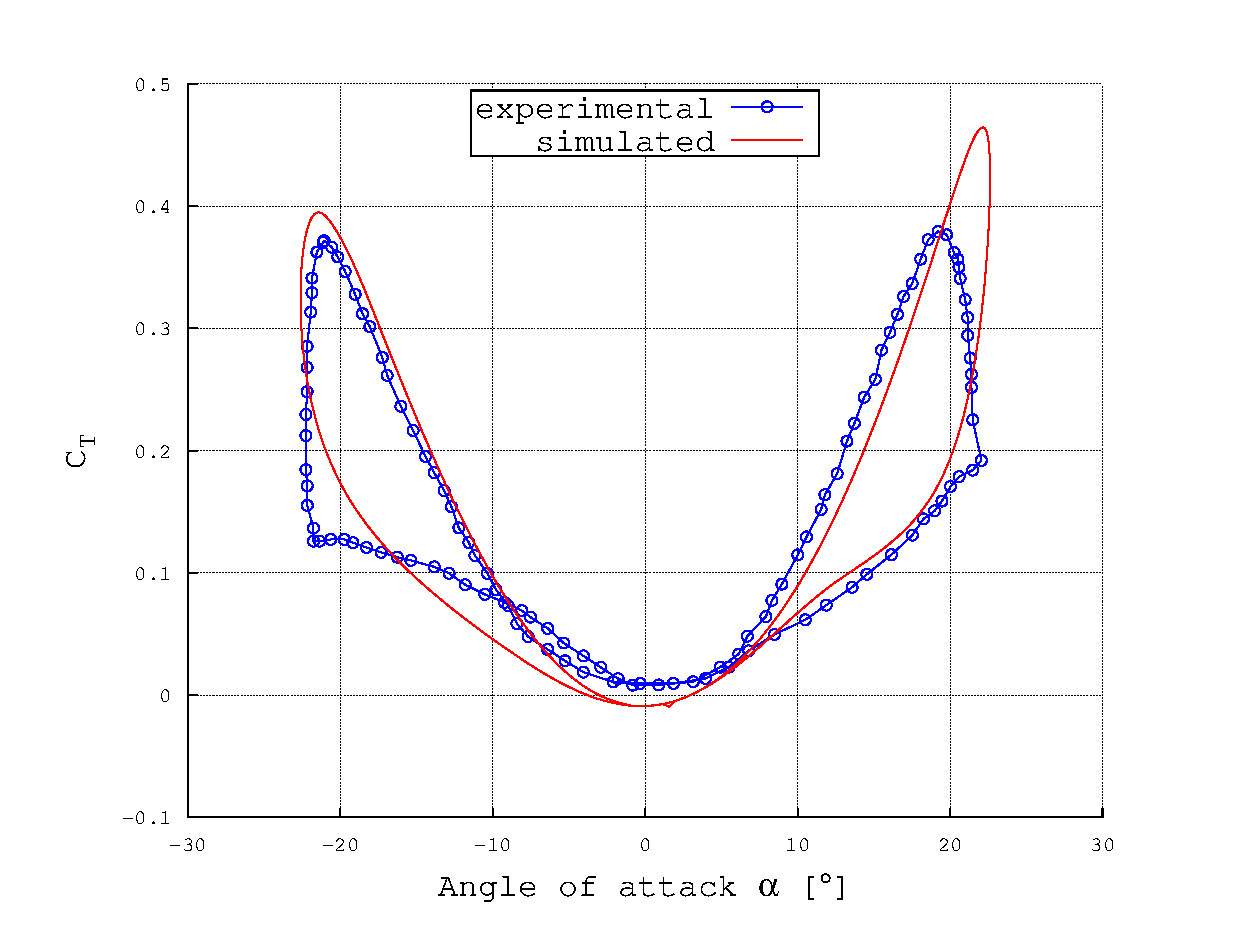
\includegraphics{CT226}}%
    \gplfronttext
  \end{picture}%
\endgroup
}
\end{minipage}
\caption{\label{fig226}Normal (left) and tangential (right) force coefficients during pitching motions of NACA0021 airfoil with a maximum amplitude of 22.6\degree\ (analog to $\lambda = 2.60$).}
\end{figure}

\subsection{Turbulence model comparison}
A simulation with a RANS $k$-$\epsilon$ standard turbulence model was carried out to compare the obtained results against another one using a LES Smagorinsky turbulence model. Figure \ref{RANSLES} shows that for the $C_N$ values there is not considerable difference, but a small improvement has been achieved for the $C_T$ values.

\begin{figure}[h]
\begin{minipage}{18pc}
\resizebox{\columnwidth}{!}{% GNUPLOT: LaTeX picture with Postscript
\begingroup
  \makeatletter
  \providecommand\color[2][]{%
    \GenericError{(gnuplot) \space\space\space\@spaces}{%
      Package color not loaded in conjunction with
      terminal option `colourtext'%
    }{See the gnuplot documentation for explanation.%
    }{Either use 'blacktext' in gnuplot or load the package
      color.sty in LaTeX.}%
    \renewcommand\color[2][]{}%
  }%
  \providecommand\includegraphics[2][]{%
    \GenericError{(gnuplot) \space\space\space\@spaces}{%
      Package graphicx or graphics not loaded%
    }{See the gnuplot documentation for explanation.%
    }{The gnuplot epslatex terminal needs graphicx.sty or graphics.sty.}%
    \renewcommand\includegraphics[2][]{}%
  }%
  \providecommand\rotatebox[2]{#2}%
  \@ifundefined{ifGPcolor}{%
    \newif\ifGPcolor
    \GPcolorfalse
  }{}%
  \@ifundefined{ifGPblacktext}{%
    \newif\ifGPblacktext
    \GPblacktexttrue
  }{}%
  % define a \g@addto@macro without @ in the name:
  \let\gplgaddtomacro\g@addto@macro
  % define empty templates for all commands taking text:
  \gdef\gplbacktext{}%
  \gdef\gplfronttext{}%
  \makeatother
  \ifGPblacktext
    % no textcolor at all
    \def\colorrgb#1{}%
    \def\colorgray#1{}%
  \else
    % gray or color?
    \ifGPcolor
      \def\colorrgb#1{\color[rgb]{#1}}%
      \def\colorgray#1{\color[gray]{#1}}%
      \expandafter\def\csname LTw\endcsname{\color{white}}%
      \expandafter\def\csname LTb\endcsname{\color{black}}%
      \expandafter\def\csname LTa\endcsname{\color{black}}%
      \expandafter\def\csname LT0\endcsname{\color[rgb]{1,0,0}}%
      \expandafter\def\csname LT1\endcsname{\color[rgb]{0,1,0}}%
      \expandafter\def\csname LT2\endcsname{\color[rgb]{0,0,1}}%
      \expandafter\def\csname LT3\endcsname{\color[rgb]{1,0,1}}%
      \expandafter\def\csname LT4\endcsname{\color[rgb]{0,1,1}}%
      \expandafter\def\csname LT5\endcsname{\color[rgb]{1,1,0}}%
      \expandafter\def\csname LT6\endcsname{\color[rgb]{0,0,0}}%
      \expandafter\def\csname LT7\endcsname{\color[rgb]{1,0.3,0}}%
      \expandafter\def\csname LT8\endcsname{\color[rgb]{0.5,0.5,0.5}}%
    \else
      % gray
      \def\colorrgb#1{\color{black}}%
      \def\colorgray#1{\color[gray]{#1}}%
      \expandafter\def\csname LTw\endcsname{\color{white}}%
      \expandafter\def\csname LTb\endcsname{\color{black}}%
      \expandafter\def\csname LTa\endcsname{\color{black}}%
      \expandafter\def\csname LT0\endcsname{\color{black}}%
      \expandafter\def\csname LT1\endcsname{\color{black}}%
      \expandafter\def\csname LT2\endcsname{\color{black}}%
      \expandafter\def\csname LT3\endcsname{\color{black}}%
      \expandafter\def\csname LT4\endcsname{\color{black}}%
      \expandafter\def\csname LT5\endcsname{\color{black}}%
      \expandafter\def\csname LT6\endcsname{\color{black}}%
      \expandafter\def\csname LT7\endcsname{\color{black}}%
      \expandafter\def\csname LT8\endcsname{\color{black}}%
    \fi
  \fi
  \setlength{\unitlength}{0.0500bp}%
  \begin{picture}(7200.00,5040.00)%
    \gplgaddtomacro\gplbacktext{%
      \csname LTb\endcsname%
      \put(946,704){\makebox(0,0)[r]{\strut{}-2}}%
      \csname LTb\endcsname%
      \put(946,1213){\makebox(0,0)[r]{\strut{}-1.5}}%
      \csname LTb\endcsname%
      \put(946,1722){\makebox(0,0)[r]{\strut{}-1}}%
      \csname LTb\endcsname%
      \put(946,2231){\makebox(0,0)[r]{\strut{}-0.5}}%
      \csname LTb\endcsname%
      \put(946,2740){\makebox(0,0)[r]{\strut{} 0}}%
      \csname LTb\endcsname%
      \put(946,3248){\makebox(0,0)[r]{\strut{} 0.5}}%
      \csname LTb\endcsname%
      \put(946,3757){\makebox(0,0)[r]{\strut{} 1}}%
      \csname LTb\endcsname%
      \put(946,4266){\makebox(0,0)[r]{\strut{} 1.5}}%
      \csname LTb\endcsname%
      \put(946,4775){\makebox(0,0)[r]{\strut{} 2}}%
      \csname LTb\endcsname%
      \put(1078,484){\makebox(0,0){\strut{}-25}}%
      \csname LTb\endcsname%
      \put(1651,484){\makebox(0,0){\strut{}-20}}%
      \csname LTb\endcsname%
      \put(2223,484){\makebox(0,0){\strut{}-15}}%
      \csname LTb\endcsname%
      \put(2796,484){\makebox(0,0){\strut{}-10}}%
      \csname LTb\endcsname%
      \put(3368,484){\makebox(0,0){\strut{}-5}}%
      \csname LTb\endcsname%
      \put(3941,484){\makebox(0,0){\strut{} 0}}%
      \csname LTb\endcsname%
      \put(4513,484){\makebox(0,0){\strut{} 5}}%
      \csname LTb\endcsname%
      \put(5086,484){\makebox(0,0){\strut{} 10}}%
      \csname LTb\endcsname%
      \put(5658,484){\makebox(0,0){\strut{} 15}}%
      \csname LTb\endcsname%
      \put(6231,484){\makebox(0,0){\strut{} 20}}%
      \csname LTb\endcsname%
      \put(6803,484){\makebox(0,0){\strut{} 25}}%
      \put(176,2739){\rotatebox{-270}{\makebox(0,0){\strut{}$C_N$}}}%
      \put(3940,154){\makebox(0,0){\strut{}Angle of attack {$\alpha$} [$\degree$]}}%
    }%
    \gplgaddtomacro\gplfronttext{%
      \csname LTb\endcsname%
      \put(2794,4602){\makebox(0,0)[r]{\strut{}experimental}}%
      \csname LTb\endcsname%
      \put(2794,4382){\makebox(0,0)[r]{\strut{}RANS}}%
      \csname LTb\endcsname%
      \put(2794,4162){\makebox(0,0)[r]{\strut{}LES}}%
    }%
    \gplbacktext
    \put(0,0){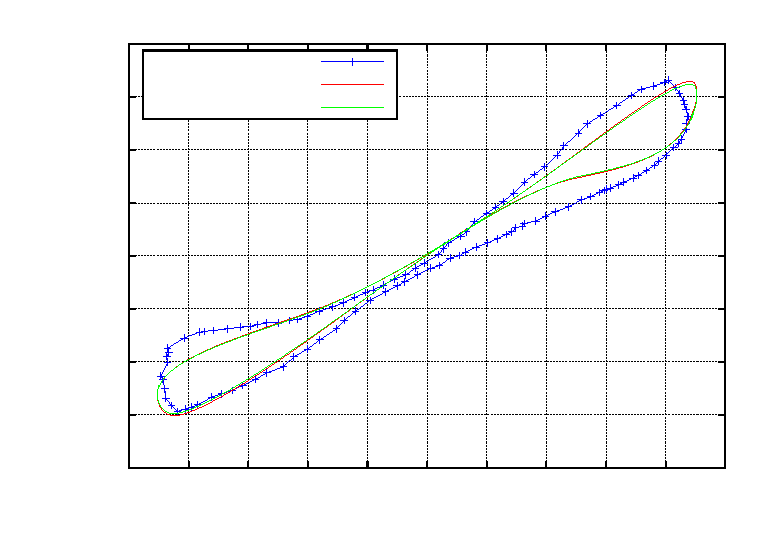
\includegraphics{CNRANSLES}}%
    \gplfronttext
  \end{picture}%
\endgroup
}
%\resizebox{\columnwidth}{!}{\input{plot}}
\end{minipage}\hspace{2pc}%
\begin{minipage}{18pc}
\resizebox{\columnwidth}{!}{% GNUPLOT: LaTeX picture with Postscript
\begingroup
  \makeatletter
  \providecommand\color[2][]{%
    \GenericError{(gnuplot) \space\space\space\@spaces}{%
      Package color not loaded in conjunction with
      terminal option `colourtext'%
    }{See the gnuplot documentation for explanation.%
    }{Either use 'blacktext' in gnuplot or load the package
      color.sty in LaTeX.}%
    \renewcommand\color[2][]{}%
  }%
  \providecommand\includegraphics[2][]{%
    \GenericError{(gnuplot) \space\space\space\@spaces}{%
      Package graphicx or graphics not loaded%
    }{See the gnuplot documentation for explanation.%
    }{The gnuplot epslatex terminal needs graphicx.sty or graphics.sty.}%
    \renewcommand\includegraphics[2][]{}%
  }%
  \providecommand\rotatebox[2]{#2}%
  \@ifundefined{ifGPcolor}{%
    \newif\ifGPcolor
    \GPcolorfalse
  }{}%
  \@ifundefined{ifGPblacktext}{%
    \newif\ifGPblacktext
    \GPblacktexttrue
  }{}%
  % define a \g@addto@macro without @ in the name:
  \let\gplgaddtomacro\g@addto@macro
  % define empty templates for all commands taking text:
  \gdef\gplbacktext{}%
  \gdef\gplfronttext{}%
  \makeatother
  \ifGPblacktext
    % no textcolor at all
    \def\colorrgb#1{}%
    \def\colorgray#1{}%
  \else
    % gray or color?
    \ifGPcolor
      \def\colorrgb#1{\color[rgb]{#1}}%
      \def\colorgray#1{\color[gray]{#1}}%
      \expandafter\def\csname LTw\endcsname{\color{white}}%
      \expandafter\def\csname LTb\endcsname{\color{black}}%
      \expandafter\def\csname LTa\endcsname{\color{black}}%
      \expandafter\def\csname LT0\endcsname{\color[rgb]{1,0,0}}%
      \expandafter\def\csname LT1\endcsname{\color[rgb]{0,1,0}}%
      \expandafter\def\csname LT2\endcsname{\color[rgb]{0,0,1}}%
      \expandafter\def\csname LT3\endcsname{\color[rgb]{1,0,1}}%
      \expandafter\def\csname LT4\endcsname{\color[rgb]{0,1,1}}%
      \expandafter\def\csname LT5\endcsname{\color[rgb]{1,1,0}}%
      \expandafter\def\csname LT6\endcsname{\color[rgb]{0,0,0}}%
      \expandafter\def\csname LT7\endcsname{\color[rgb]{1,0.3,0}}%
      \expandafter\def\csname LT8\endcsname{\color[rgb]{0.5,0.5,0.5}}%
    \else
      % gray
      \def\colorrgb#1{\color{black}}%
      \def\colorgray#1{\color[gray]{#1}}%
      \expandafter\def\csname LTw\endcsname{\color{white}}%
      \expandafter\def\csname LTb\endcsname{\color{black}}%
      \expandafter\def\csname LTa\endcsname{\color{black}}%
      \expandafter\def\csname LT0\endcsname{\color{black}}%
      \expandafter\def\csname LT1\endcsname{\color{black}}%
      \expandafter\def\csname LT2\endcsname{\color{black}}%
      \expandafter\def\csname LT3\endcsname{\color{black}}%
      \expandafter\def\csname LT4\endcsname{\color{black}}%
      \expandafter\def\csname LT5\endcsname{\color{black}}%
      \expandafter\def\csname LT6\endcsname{\color{black}}%
      \expandafter\def\csname LT7\endcsname{\color{black}}%
      \expandafter\def\csname LT8\endcsname{\color{black}}%
    \fi
  \fi
  \setlength{\unitlength}{0.0500bp}%
  \begin{picture}(7200.00,5040.00)%
    \gplgaddtomacro\gplbacktext{%
      \csname LTb\endcsname%
      \put(1078,704){\makebox(0,0)[r]{\strut{}-0.05}}%
      \csname LTb\endcsname%
      \put(1078,1074){\makebox(0,0)[r]{\strut{} 0}}%
      \csname LTb\endcsname%
      \put(1078,1444){\makebox(0,0)[r]{\strut{} 0.05}}%
      \csname LTb\endcsname%
      \put(1078,1814){\makebox(0,0)[r]{\strut{} 0.1}}%
      \csname LTb\endcsname%
      \put(1078,2184){\makebox(0,0)[r]{\strut{} 0.15}}%
      \csname LTb\endcsname%
      \put(1078,2554){\makebox(0,0)[r]{\strut{} 0.2}}%
      \csname LTb\endcsname%
      \put(1078,2925){\makebox(0,0)[r]{\strut{} 0.25}}%
      \csname LTb\endcsname%
      \put(1078,3295){\makebox(0,0)[r]{\strut{} 0.3}}%
      \csname LTb\endcsname%
      \put(1078,3665){\makebox(0,0)[r]{\strut{} 0.35}}%
      \csname LTb\endcsname%
      \put(1078,4035){\makebox(0,0)[r]{\strut{} 0.4}}%
      \csname LTb\endcsname%
      \put(1078,4405){\makebox(0,0)[r]{\strut{} 0.45}}%
      \csname LTb\endcsname%
      \put(1078,4775){\makebox(0,0)[r]{\strut{} 0.5}}%
      \csname LTb\endcsname%
      \put(1210,484){\makebox(0,0){\strut{}-25}}%
      \csname LTb\endcsname%
      \put(1769,484){\makebox(0,0){\strut{}-20}}%
      \csname LTb\endcsname%
      \put(2329,484){\makebox(0,0){\strut{}-15}}%
      \csname LTb\endcsname%
      \put(2888,484){\makebox(0,0){\strut{}-10}}%
      \csname LTb\endcsname%
      \put(3447,484){\makebox(0,0){\strut{}-5}}%
      \csname LTb\endcsname%
      \put(4007,484){\makebox(0,0){\strut{} 0}}%
      \csname LTb\endcsname%
      \put(4566,484){\makebox(0,0){\strut{} 5}}%
      \csname LTb\endcsname%
      \put(5125,484){\makebox(0,0){\strut{} 10}}%
      \csname LTb\endcsname%
      \put(5684,484){\makebox(0,0){\strut{} 15}}%
      \csname LTb\endcsname%
      \put(6244,484){\makebox(0,0){\strut{} 20}}%
      \csname LTb\endcsname%
      \put(6803,484){\makebox(0,0){\strut{} 25}}%
      \put(176,2739){\rotatebox{-270}{\makebox(0,0){\strut{}$C_T$}}}%
      \put(4006,154){\makebox(0,0){\strut{}Angle of attack {$\alpha$} [$\degree$]}}%
    }%
    \gplgaddtomacro\gplfronttext{%
      \csname LTb\endcsname%
      \put(4371,4602){\makebox(0,0)[r]{\strut{}experimental}}%
      \csname LTb\endcsname%
      \put(4371,4382){\makebox(0,0)[r]{\strut{}RANS}}%
      \csname LTb\endcsname%
      \put(4371,4162){\makebox(0,0)[r]{\strut{}LES}}%
    }%
    \gplbacktext
    \put(0,0){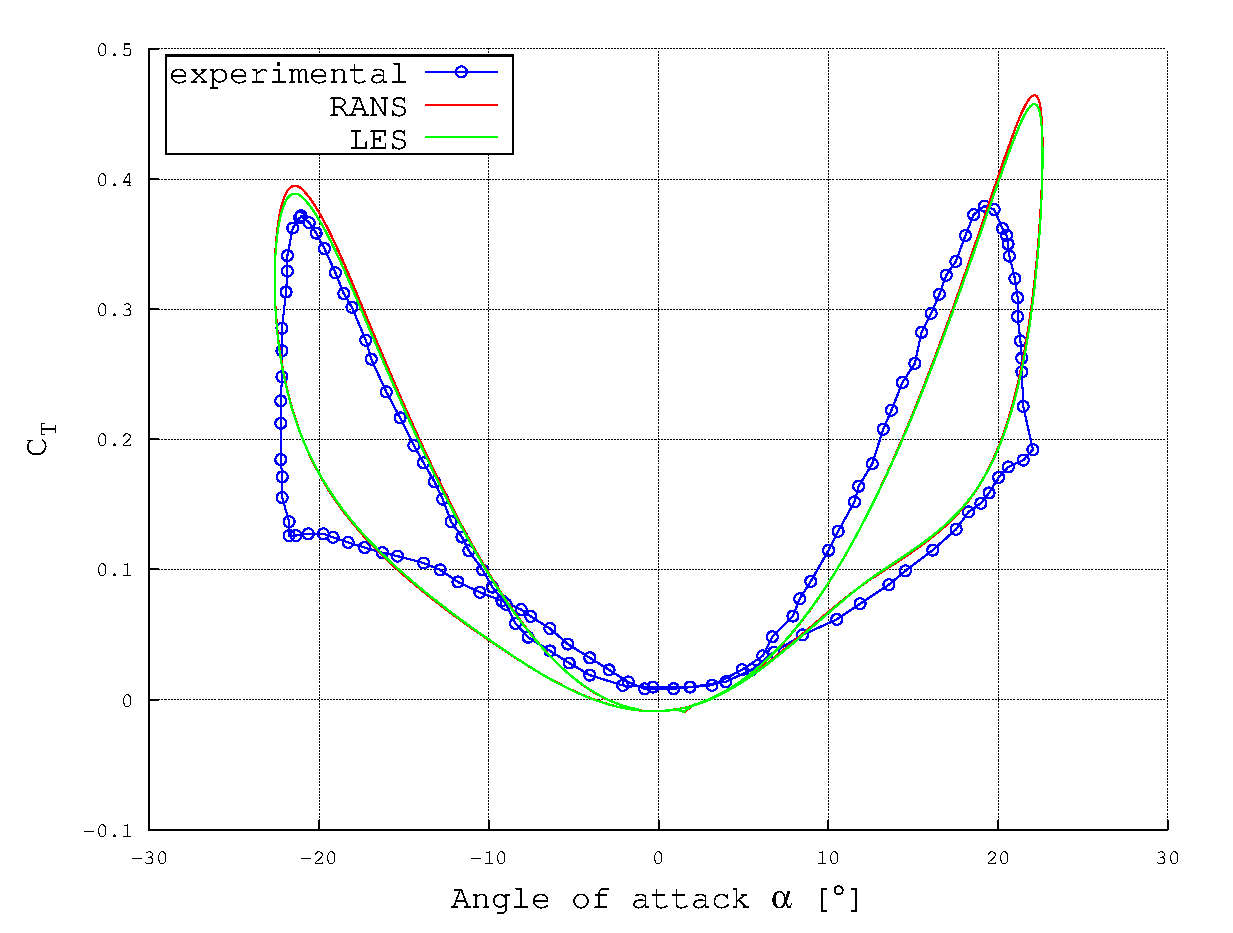
\includegraphics{CTRANSLES}}%
    \gplfronttext
  \end{picture}%
\endgroup
}
\end{minipage}
\caption{\label{RANSLES}Normal (left) and tangential (right) force coefficients for different turbulence models, pithing motion with a maximum amplitude of 22.6\degree\ }
\end{figure}

\subsection{Unsteady effects correction}
A test for the simulation with the DSM turned off was carried out, it means there is no compensation for the unsteady effects: the effective angle of attack is the angle of attack provided by the ALM. Figure \ref{AMP174corrections} depicts that simulated results are closer to experimental data with the corrections. Both $C_N$ and $C_T$ peak values are not overestimated. The $C_N$ loop, shows that the model without the corrections was not able to capture reattachment flow effects.

\begin{figure}[h]
\begin{minipage}{18pc}
\resizebox{\columnwidth}{!}{% GNUPLOT: LaTeX picture with Postscript
\begingroup
  \makeatletter
  \providecommand\color[2][]{%
    \GenericError{(gnuplot) \space\space\space\@spaces}{%
      Package color not loaded in conjunction with
      terminal option `colourtext'%
    }{See the gnuplot documentation for explanation.%
    }{Either use 'blacktext' in gnuplot or load the package
      color.sty in LaTeX.}%
    \renewcommand\color[2][]{}%
  }%
  \providecommand\includegraphics[2][]{%
    \GenericError{(gnuplot) \space\space\space\@spaces}{%
      Package graphicx or graphics not loaded%
    }{See the gnuplot documentation for explanation.%
    }{The gnuplot epslatex terminal needs graphicx.sty or graphics.sty.}%
    \renewcommand\includegraphics[2][]{}%
  }%
  \providecommand\rotatebox[2]{#2}%
  \@ifundefined{ifGPcolor}{%
    \newif\ifGPcolor
    \GPcolorfalse
  }{}%
  \@ifundefined{ifGPblacktext}{%
    \newif\ifGPblacktext
    \GPblacktexttrue
  }{}%
  % define a \g@addto@macro without @ in the name:
  \let\gplgaddtomacro\g@addto@macro
  % define empty templates for all commands taking text:
  \gdef\gplbacktext{}%
  \gdef\gplfronttext{}%
  \makeatother
  \ifGPblacktext
    % no textcolor at all
    \def\colorrgb#1{}%
    \def\colorgray#1{}%
  \else
    % gray or color?
    \ifGPcolor
      \def\colorrgb#1{\color[rgb]{#1}}%
      \def\colorgray#1{\color[gray]{#1}}%
      \expandafter\def\csname LTw\endcsname{\color{white}}%
      \expandafter\def\csname LTb\endcsname{\color{black}}%
      \expandafter\def\csname LTa\endcsname{\color{black}}%
      \expandafter\def\csname LT0\endcsname{\color[rgb]{1,0,0}}%
      \expandafter\def\csname LT1\endcsname{\color[rgb]{0,1,0}}%
      \expandafter\def\csname LT2\endcsname{\color[rgb]{0,0,1}}%
      \expandafter\def\csname LT3\endcsname{\color[rgb]{1,0,1}}%
      \expandafter\def\csname LT4\endcsname{\color[rgb]{0,1,1}}%
      \expandafter\def\csname LT5\endcsname{\color[rgb]{1,1,0}}%
      \expandafter\def\csname LT6\endcsname{\color[rgb]{0,0,0}}%
      \expandafter\def\csname LT7\endcsname{\color[rgb]{1,0.3,0}}%
      \expandafter\def\csname LT8\endcsname{\color[rgb]{0.5,0.5,0.5}}%
    \else
      % gray
      \def\colorrgb#1{\color{black}}%
      \def\colorgray#1{\color[gray]{#1}}%
      \expandafter\def\csname LTw\endcsname{\color{white}}%
      \expandafter\def\csname LTb\endcsname{\color{black}}%
      \expandafter\def\csname LTa\endcsname{\color{black}}%
      \expandafter\def\csname LT0\endcsname{\color{black}}%
      \expandafter\def\csname LT1\endcsname{\color{black}}%
      \expandafter\def\csname LT2\endcsname{\color{black}}%
      \expandafter\def\csname LT3\endcsname{\color{black}}%
      \expandafter\def\csname LT4\endcsname{\color{black}}%
      \expandafter\def\csname LT5\endcsname{\color{black}}%
      \expandafter\def\csname LT6\endcsname{\color{black}}%
      \expandafter\def\csname LT7\endcsname{\color{black}}%
      \expandafter\def\csname LT8\endcsname{\color{black}}%
    \fi
  \fi
  \setlength{\unitlength}{0.0500bp}%
  \begin{picture}(7200.00,5040.00)%
    \gplgaddtomacro\gplbacktext{%
      \csname LTb\endcsname%
      \put(946,704){\makebox(0,0)[r]{\strut{}-1.5}}%
      \csname LTb\endcsname%
      \put(946,1383){\makebox(0,0)[r]{\strut{}-1}}%
      \csname LTb\endcsname%
      \put(946,2061){\makebox(0,0)[r]{\strut{}-0.5}}%
      \csname LTb\endcsname%
      \put(946,2740){\makebox(0,0)[r]{\strut{} 0}}%
      \csname LTb\endcsname%
      \put(946,3418){\makebox(0,0)[r]{\strut{} 0.5}}%
      \csname LTb\endcsname%
      \put(946,4097){\makebox(0,0)[r]{\strut{} 1}}%
      \csname LTb\endcsname%
      \put(946,4775){\makebox(0,0)[r]{\strut{} 1.5}}%
      \csname LTb\endcsname%
      \put(1078,484){\makebox(0,0){\strut{}-20}}%
      \csname LTb\endcsname%
      \put(1794,484){\makebox(0,0){\strut{}-15}}%
      \csname LTb\endcsname%
      \put(2509,484){\makebox(0,0){\strut{}-10}}%
      \csname LTb\endcsname%
      \put(3225,484){\makebox(0,0){\strut{}-5}}%
      \csname LTb\endcsname%
      \put(3941,484){\makebox(0,0){\strut{} 0}}%
      \csname LTb\endcsname%
      \put(4656,484){\makebox(0,0){\strut{} 5}}%
      \csname LTb\endcsname%
      \put(5372,484){\makebox(0,0){\strut{} 10}}%
      \csname LTb\endcsname%
      \put(6087,484){\makebox(0,0){\strut{} 15}}%
      \csname LTb\endcsname%
      \put(6803,484){\makebox(0,0){\strut{} 20}}%
      \put(176,2739){\rotatebox{-270}{\makebox(0,0){\strut{}$C_N$}}}%
      \put(3940,154){\makebox(0,0){\strut{}Angle of attack {$\alpha$} [$\degree$]}}%
    }%
    \gplgaddtomacro\gplfronttext{%
      \csname LTb\endcsname%
      \put(2794,4602){\makebox(0,0)[r]{\strut{}experimental}}%
      \csname LTb\endcsname%
      \put(2794,4382){\makebox(0,0)[r]{\strut{}DSM on}}%
      \csname LTb\endcsname%
      \put(2794,4162){\makebox(0,0)[r]{\strut{}DSM off}}%
    }%
    \gplbacktext
    \put(0,0){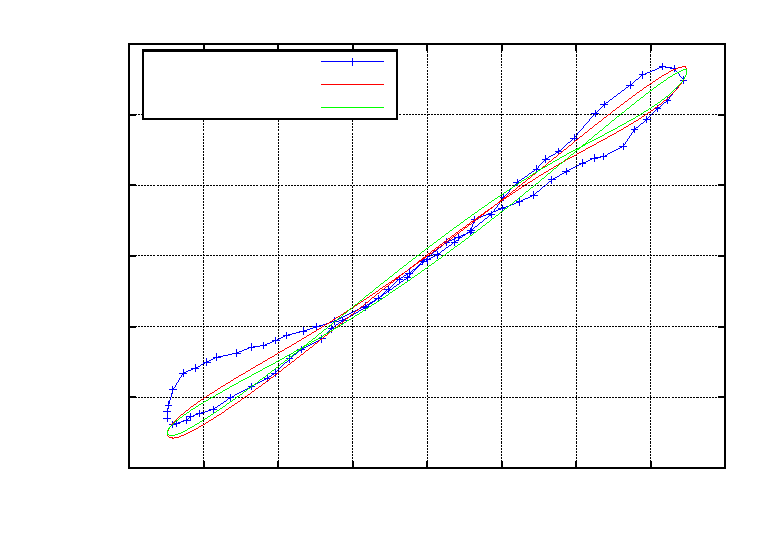
\includegraphics{CNAMP174corrections}}%
    \gplfronttext
  \end{picture}%
\endgroup
}
%\resizebox{\columnwidth}{!}{\input{plot}}
\end{minipage}\hspace{2pc}%
\begin{minipage}{18pc}
\resizebox{\columnwidth}{!}{% GNUPLOT: LaTeX picture with Postscript
\begingroup
  \makeatletter
  \providecommand\color[2][]{%
    \GenericError{(gnuplot) \space\space\space\@spaces}{%
      Package color not loaded in conjunction with
      terminal option `colourtext'%
    }{See the gnuplot documentation for explanation.%
    }{Either use 'blacktext' in gnuplot or load the package
      color.sty in LaTeX.}%
    \renewcommand\color[2][]{}%
  }%
  \providecommand\includegraphics[2][]{%
    \GenericError{(gnuplot) \space\space\space\@spaces}{%
      Package graphicx or graphics not loaded%
    }{See the gnuplot documentation for explanation.%
    }{The gnuplot epslatex terminal needs graphicx.sty or graphics.sty.}%
    \renewcommand\includegraphics[2][]{}%
  }%
  \providecommand\rotatebox[2]{#2}%
  \@ifundefined{ifGPcolor}{%
    \newif\ifGPcolor
    \GPcolorfalse
  }{}%
  \@ifundefined{ifGPblacktext}{%
    \newif\ifGPblacktext
    \GPblacktexttrue
  }{}%
  % define a \g@addto@macro without @ in the name:
  \let\gplgaddtomacro\g@addto@macro
  % define empty templates for all commands taking text:
  \gdef\gplbacktext{}%
  \gdef\gplfronttext{}%
  \makeatother
  \ifGPblacktext
    % no textcolor at all
    \def\colorrgb#1{}%
    \def\colorgray#1{}%
  \else
    % gray or color?
    \ifGPcolor
      \def\colorrgb#1{\color[rgb]{#1}}%
      \def\colorgray#1{\color[gray]{#1}}%
      \expandafter\def\csname LTw\endcsname{\color{white}}%
      \expandafter\def\csname LTb\endcsname{\color{black}}%
      \expandafter\def\csname LTa\endcsname{\color{black}}%
      \expandafter\def\csname LT0\endcsname{\color[rgb]{1,0,0}}%
      \expandafter\def\csname LT1\endcsname{\color[rgb]{0,1,0}}%
      \expandafter\def\csname LT2\endcsname{\color[rgb]{0,0,1}}%
      \expandafter\def\csname LT3\endcsname{\color[rgb]{1,0,1}}%
      \expandafter\def\csname LT4\endcsname{\color[rgb]{0,1,1}}%
      \expandafter\def\csname LT5\endcsname{\color[rgb]{1,1,0}}%
      \expandafter\def\csname LT6\endcsname{\color[rgb]{0,0,0}}%
      \expandafter\def\csname LT7\endcsname{\color[rgb]{1,0.3,0}}%
      \expandafter\def\csname LT8\endcsname{\color[rgb]{0.5,0.5,0.5}}%
    \else
      % gray
      \def\colorrgb#1{\color{black}}%
      \def\colorgray#1{\color[gray]{#1}}%
      \expandafter\def\csname LTw\endcsname{\color{white}}%
      \expandafter\def\csname LTb\endcsname{\color{black}}%
      \expandafter\def\csname LTa\endcsname{\color{black}}%
      \expandafter\def\csname LT0\endcsname{\color{black}}%
      \expandafter\def\csname LT1\endcsname{\color{black}}%
      \expandafter\def\csname LT2\endcsname{\color{black}}%
      \expandafter\def\csname LT3\endcsname{\color{black}}%
      \expandafter\def\csname LT4\endcsname{\color{black}}%
      \expandafter\def\csname LT5\endcsname{\color{black}}%
      \expandafter\def\csname LT6\endcsname{\color{black}}%
      \expandafter\def\csname LT7\endcsname{\color{black}}%
      \expandafter\def\csname LT8\endcsname{\color{black}}%
    \fi
  \fi
  \setlength{\unitlength}{0.0500bp}%
  \begin{picture}(7200.00,5040.00)%
    \gplgaddtomacro\gplbacktext{%
      \csname LTb\endcsname%
      \put(1078,704){\makebox(0,0)[r]{\strut{}-0.05}}%
      \csname LTb\endcsname%
      \put(1078,1286){\makebox(0,0)[r]{\strut{} 0}}%
      \csname LTb\endcsname%
      \put(1078,1867){\makebox(0,0)[r]{\strut{} 0.05}}%
      \csname LTb\endcsname%
      \put(1078,2449){\makebox(0,0)[r]{\strut{} 0.1}}%
      \csname LTb\endcsname%
      \put(1078,3030){\makebox(0,0)[r]{\strut{} 0.15}}%
      \csname LTb\endcsname%
      \put(1078,3612){\makebox(0,0)[r]{\strut{} 0.2}}%
      \csname LTb\endcsname%
      \put(1078,4193){\makebox(0,0)[r]{\strut{} 0.25}}%
      \csname LTb\endcsname%
      \put(1078,4775){\makebox(0,0)[r]{\strut{} 0.3}}%
      \csname LTb\endcsname%
      \put(1210,484){\makebox(0,0){\strut{}-20}}%
      \csname LTb\endcsname%
      \put(1909,484){\makebox(0,0){\strut{}-15}}%
      \csname LTb\endcsname%
      \put(2608,484){\makebox(0,0){\strut{}-10}}%
      \csname LTb\endcsname%
      \put(3307,484){\makebox(0,0){\strut{}-5}}%
      \csname LTb\endcsname%
      \put(4007,484){\makebox(0,0){\strut{} 0}}%
      \csname LTb\endcsname%
      \put(4706,484){\makebox(0,0){\strut{} 5}}%
      \csname LTb\endcsname%
      \put(5405,484){\makebox(0,0){\strut{} 10}}%
      \csname LTb\endcsname%
      \put(6104,484){\makebox(0,0){\strut{} 15}}%
      \csname LTb\endcsname%
      \put(6803,484){\makebox(0,0){\strut{} 20}}%
      \put(176,2739){\rotatebox{-270}{\makebox(0,0){\strut{}$C_T$}}}%
      \put(4006,154){\makebox(0,0){\strut{}Angle of attack {$\alpha$} [$\degree$]}}%
    }%
    \gplgaddtomacro\gplfronttext{%
      \csname LTb\endcsname%
      \put(4371,4602){\makebox(0,0)[r]{\strut{}experimental}}%
      \csname LTb\endcsname%
      \put(4371,4382){\makebox(0,0)[r]{\strut{}DSM on}}%
      \csname LTb\endcsname%
      \put(4371,4162){\makebox(0,0)[r]{\strut{}DSM off}}%
    }%
    \gplbacktext
    \put(0,0){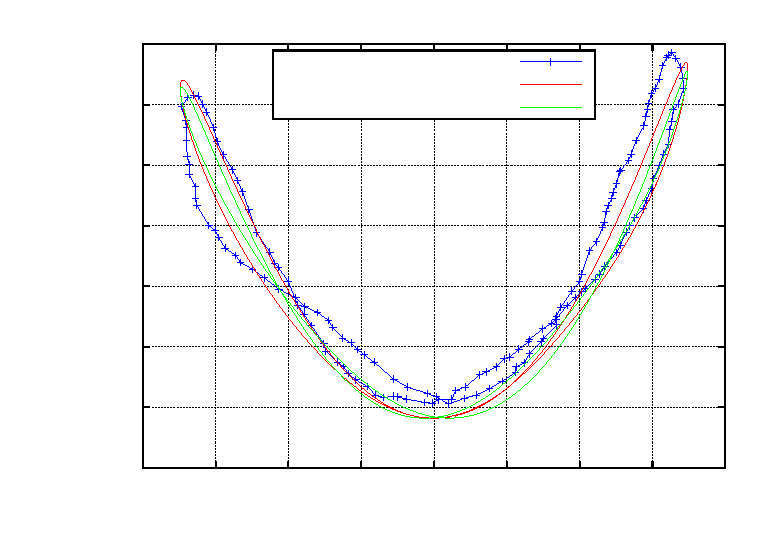
\includegraphics{CTAMP174corrections}}%
    \gplfronttext
  \end{picture}%
\endgroup
}
\end{minipage}
\caption{\label{AMP174corrections}Normal (left) and tangential (right) force coefficients with and without unsteady effects correction, pithing motion with a maximum amplitude of 17.4\degree\ }
\end{figure}


\section{Conclusions}

It has been demonstrated that the presented coupled model ALM with DSM, shows
good agreement with experimental data, considering the complexity of the flows
studied. Moreover, the model has been tested for a wide range of pithing
amplitudes, therefore, with different stall conditions (none, shallow, and deep
stall), results agreed well compared with experiments. The model is stable and
accurate for the tested pithing blade motions, which makes it suitable for
application in VAT simulations.


\section*{Acknowledgment}
Financial support from STandUP for Energy and Uppsala University, are gratefully acknowledged.


\section*{References}

\bibliography{mybib}{}
\bibliographystyle{unsrt}


\end{document}
